\documentclass[12pt]{article}
\usepackage[utf8]{inputenc}
\usepackage[usenames]{color}
\usepackage[margin=1in]{geometry} 
\usepackage{amsmath,amsthm,amssymb,graphicx,mathtools,tikz,hyperref, pgfplots, listings, pdfpages}
\usetikzlibrary{positioning}
\newcommand{\n}{\mathbb{N}}
\newcommand{\z}{\mathbb{Z}}
\newcommand{\q}{\mathbb{Q}}
\newcommand{\cx}{\mathbb{C}}
\newcommand{\real}{\mathbb{R}}
\newcommand{\field}{\mathbb{F}}
\newcommand{\ita}[1]{\textit{#1}}
\newcommand{\com}[2]{#1\backslash#2}
\newcommand{\oneton}{\{1,2,3,...,n\}}
\newcommand\idea[1]{\begin{gather*}#1\end{gather*}}
\newcommand\ef{\ita{f} }
\newcommand\eff{\ita{f}}
\newcommand\proofs[1]{\begin{proof}#1\end{proof}}
\newcommand\inv[1]{#1^{-1}}
\newcommand\setb[1]{\{#1\}}
\newcommand\en{\ita{n }}
\newcommand{\vbrack}[1]{\langle #1\rangle}


\newenvironment{theorem}[2][Teorema]{\begin{trivlist}
\item[\hskip \labelsep {\bfseries #1}\hskip \labelsep {\bfseries #2.}]}{\end{trivlist}}
\newenvironment{lemma}[2][Lema]{\begin{trivlist}
\item[\hskip \labelsep {\bfseries #1}\hskip \labelsep {\bfseries #2.}]}{\end{trivlist}}
\newenvironment{exercise}[2][Ejercicio]{\begin{trivlist}
\item[\hskip \labelsep {\bfseries #1}\hskip \labelsep {\bfseries #2.}]}{\end{trivlist}}
\newenvironment{reflection}[2][Reflexión]{\begin{trivlist}
\item[\hskip \labelsep {\bfseries #1}\hskip \labelsep {\bfseries #2.}]}{\end{trivlist}}
\newenvironment{proposition}[2][Proposición]{\begin{trivlist}
\item[\hskip \labelsep {\bfseries #1}\hskip \labelsep {\bfseries #2.}]}{\end{trivlist}}
\newenvironment{corollary}[2][Corolario]{\begin{trivlist}
\item[\hskip \labelsep {\bfseries #1}\hskip \labelsep {\bfseries #2.}]}{\end{trivlist}}
 \hypersetup{
 colorlinks,
 linkcolor=blue
 }

\renewcommand{\ttdefault}{pcr}
\lstdefinestyle{C}{language=C,
    basicstyle=\ttfamily,
    keywordstyle=\bfseries,
    showstringspaces=false,
    morekeywords={include, printf},
	keepspaces=true,numbers=left,xleftmargin=2em,frame=shadowbox,framexleftmargin=0 em, rulesepcolor = \color{black}
}
\lstdefinestyle{linuxterminal}{language=bash,
    basicstyle=\ttfamily,
    keywordstyle=\bfseries,
    showstringspaces=false,
    morekeywords={include, printf},
	keepspaces=true,
	frame=TLRB
}

\begin{document}
	\date{15-02-2018}
	
	
	\title{\textbf{\textcolor{red}{REQUIREMENTS ANALYSIS DOCUMENT}}}
	\author{Alejandro Santorum Varela - alejandro.santorum@estudiante.uam.es\\David Cabornero Pascual - david.cabornero@estudiante.uam.es\\Autonomous University of Madrid}
	\maketitle
	
\tableofcontents

\section{Introduction}
\subsection{Purpose of the system}
The proposed application is called "PhotoHouse". It allows users to find apartments or stays that are available to be rented.\\\\
This application aims to be the first means of connection between the landlord and the customer.\\\\
There are different types of users, depending on the registration, that have not got the same permits. They are going to be explained  later wider. Depending on the user type, you will be able to filter offers with postal code, stay type, range of dates, puntuation, price and state of the offer.\\\\
There are mainly two types of stays: short period of stays and long stays. You can also differenciate an offer by its cost, its location, its puntuation, its description and some other stuff.\\\\
The payments are performed through a auxiliary application. PhotoHouse gets the 2\% of the offer price in its advantage, and 0.1\% in long stays. The rest is logically given to the landlord.\\\\

\subsection{Scope of the system}
PhotoHouse is an application that can be used by three different types of users: public users, registered users and managers. Registered users are divided at the same time in customers, landlords and customers-landlords.\\It is important to underline that the application has \textbf{not} got registration system, all the registered users are already known. However, registered users have had to provide the following information and it \textbf{cannot be changed}, but credit card number:\\
· Name\\· ID(such as TIN)\\· Password\\· Kind of user\\· Credit card number\\All users are going to be described more precisely in section \ref{subsec:fr}.\\\\
How we have said in the previous section, there exists a filter, that depending on the user driving the application, can specify the shown offers by postal code, type of stay (short or long stay), range of dates, price, puntuation and state of the offer(rented, reserved and free).\\\\
We are explaining now the posting process by which an offer is published.\\First, the landlord has to register an accommodation giving the following information, which \textbf{cannot be changed later}:\\
· Location: including address, postal code and city.\\
· Description of the accommodation.\\
· Other features and observations.\\
Next, the landlord can put in rent any property that he has registered before, giving again more information but now this info is changable:\\
· Price.\\
· Type of stay: short period stays and long period stays. Short stays are only rented between the given dates (inital date and final date), both included, and this period is not modifiable. Long stays are undefined but it is not rentable for a shorter period than the minimum period of time, the limit that differenciates short and long stays. In the case of long stays, this application eases the first payment (usually the first month) but the rest are made between landlord and customer on their own.\\
· Renting range of dates: initial date + final date in the case of short stays and minimum period of time for long stays.\\\\
Then, the manager is the responsible of approving the different offers. He can approve it or deny it.\\Once an offer is approved, it is ready to be rented.\\\\
To clarify all this process a graphic has been made:\\
\begin{center}
	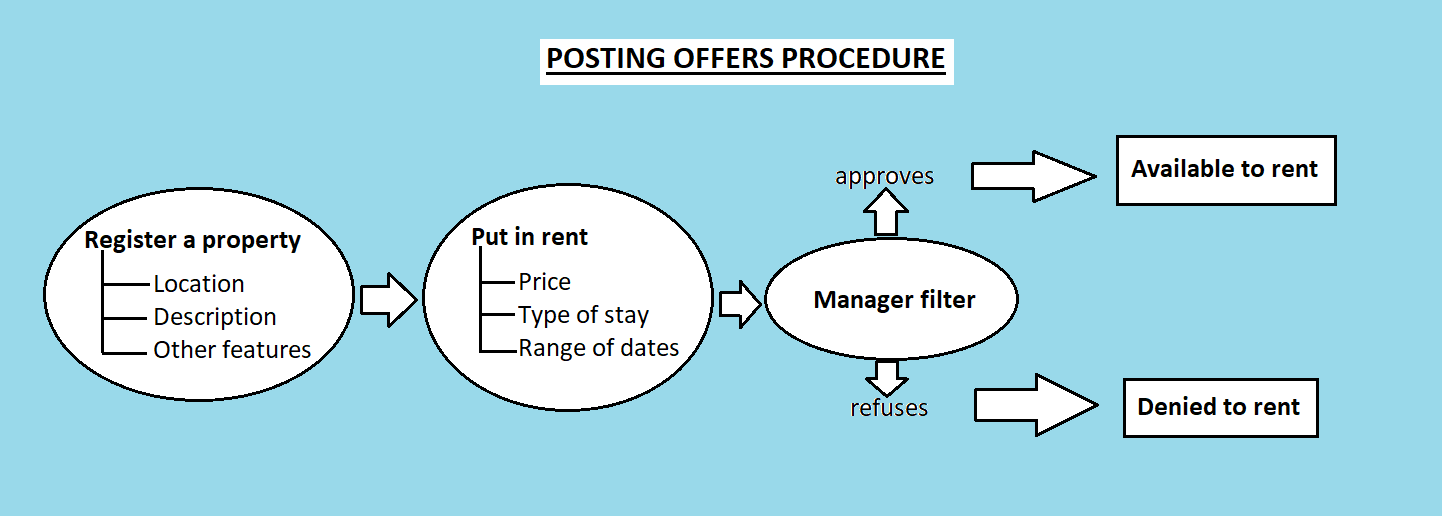
\includegraphics[scale=0.8]{posting_procedure.png}
\end{center}
Registered users can comment on the various accommodations that are visible in the application, allowing other registered users to have an idea of the apartment and feeding the ranking filter.\\\\

There is the chance to reserve an accommodation for 5 days, so nobody can rent it in those 5 days and the user can use this time to think if he/she wants to rent or not. There is no booking limitation.\\\\

Last but not least, let's talk about the payment procedure. Once a user rents an accommodation, PhotoHouse uses his/her credit card to pay the landlord, charging in form of commissions the 2\% of the price in short stays and 0.1\% of the price in long stays.\\\\
If the external application that PhotoHouse uses to charge the payment cannot perform the transference correctly, an error occurs and the user is blocked with the only allowed action to send a message to the manager in order to change the credit card number.\\\\When the customer completes the payment correctly, the apartment is rented. If there is any error at giving the money to the landlord, PhotoHouse saves all the money until the landlord changes its credit card number.\\

\subsection{Objectives and success criteria of the project}
The goals of the application, and the criteria used to decide whether the system has been built successfully, depends upon meeting the following core sets of objectives:\\
· Public users must be able to browse through the offers, but without seeing/commeting and without the possibility to rent.\\
· The application has to be able to allow landlords to register a property, offer it if it complies with the expectations, and earn money if any of their buildings have been rented.\\
· On the other hand, PhotoHouse has to permit customers to rent any accommodation if they can afford it, that is to say, if they have enough money in their credit card. Additionally, the system has to permit customers to reserve any free property for five entirely days.\\
· If there is any setback at performancing the payment, the application takes control and blocks the customer, only allowing him to contact to the manager to change its credit card number.\\
· Managers must be able to approve and refuse offers. In addiction, they must be able to modify users' credit card numbers.\\
· The system has also to provide a good commenting system, that allows registered users to evaluate any stay.\\


\subsection{Definitions, acronyms, and abbreviations}
\subsubsection{Definitions}
\underline{Customer}: A person who buys a service. In this case, a user who can rent an accommodation.\\
\underline{Landlord}: A person who owns a building or an accommodation and is paid by other people for the use of it.\\
\underline{Manager}: Also named as Administrator. A person who is responsible of managing the application, above all, approving or refusing the new offers before they are available for the rest of the users.\\
\underline{Customer-Landlord or Landlord-Customer}: In the case of this application, person who can either rent or offer an apartment/stay.
\subsubsection{Acronyms}
\underline{TIN}: acronym of Tax Identification Number.\\
\subsubsection{Abbreviations}
\underline{Postal Code}: it can be abbreviated using P.C.\\
\underline{Info}: information.\\

\section{System Description}
\subsection{Functional Requirements}{\label{subsec:fr}
How it has been said before, there exist different types of users depending on what the user want to do:
\subsubsection{Non-Registered User or Public User}
· It is the user with the least privileges.\\
· Search by type of stay (short period stay or long stay).\\
· Search by P.C.\\
· Search by range of dates.
\subsubsection{Registered User}
· Use all filters that non-registered users have.\\
· Search by price.\\
· Search by apartment's puntuation.\\
· Search by state of the offer(rented, reserved, free).\\
· Contact to a manager in order to change its credit card number.\\
· Write and read comments.\\\
· Evaluate with the puntuation system a stay.\\
· See all comments of other registered users.\\
In addiction, registered users are divided in three different types depending on it's goal:\\

\textbf{\underline{Customer:}}\\
· Rent an apartment.\\
· Reserve an apartment for five entirely days, it means no other user can rent this accommodation. There is no limit of reservations that an user can make.\\

\textbf{\underline{Landlord:}}\\
· Register a property.\\
· Try to make an offer of a property that it's already registered by the user.\\
· Edit the parameters of an offer (price, range of dates and type).\\

\textbf{\underline{Landlord+Customer:}}\\
· This user has all functions that customer, landlord and public users have.

\subsubsection{Manager}
· Approve an offer, so it is now available to be rented.\\
· Change registered users' credit card numbers.

\subsection{Non-functional Requirements}
\subsubsection{Usability}
The PhotoHouse application must be capable of supporting mouse-driven interaction as well as keyboard interaction, to broaden the user base.\\\\
Most of the cases the user will be able to communicate with the application system just clicking on the different buttoms that will be placed all over the screen with a descriptive and intuitive name. That's why we are implementing mouse-driven facilities. Another feature that would be grateful it's to scroll through the distinctive offers that will be displayed on the screen.\\\\
Finally, the keyboard will be used to write several statements, such as the login information, stays' descriptions and comments. 
\subsubsection{Reliability}
The application should be able to display a lot of offers at the same time.\\ In addiction, it must have a really good database or information container, because of the fact the rented appartements are not deleted, they are kept in the application even though the offer is finished.
\subsubsection{Performance}
User should incur very little penalty.\\ It is obvious the more apartments are printed, the more the system degrades, but it won't be a perceptible problem. Anyway, the user can select the shown accommodations just reforcing the parameters of the filter.
\subsubsection{Supportability}
It is design to be run in Windows O.S., especially Windows 10.
\subsubsection{Implementation}
It is going to be implemented with Java Programming Language, using either a programmer's text editor or either a IDE such as Eclipse.\\\\ Graphically speaking, it will be probably programmed using Java API for graphical entities known as the Java Advanced Windowing Toolkit (AWT).\\
\section{Use Cases}
\subsection{Use Case diagram}
\begin{center}
	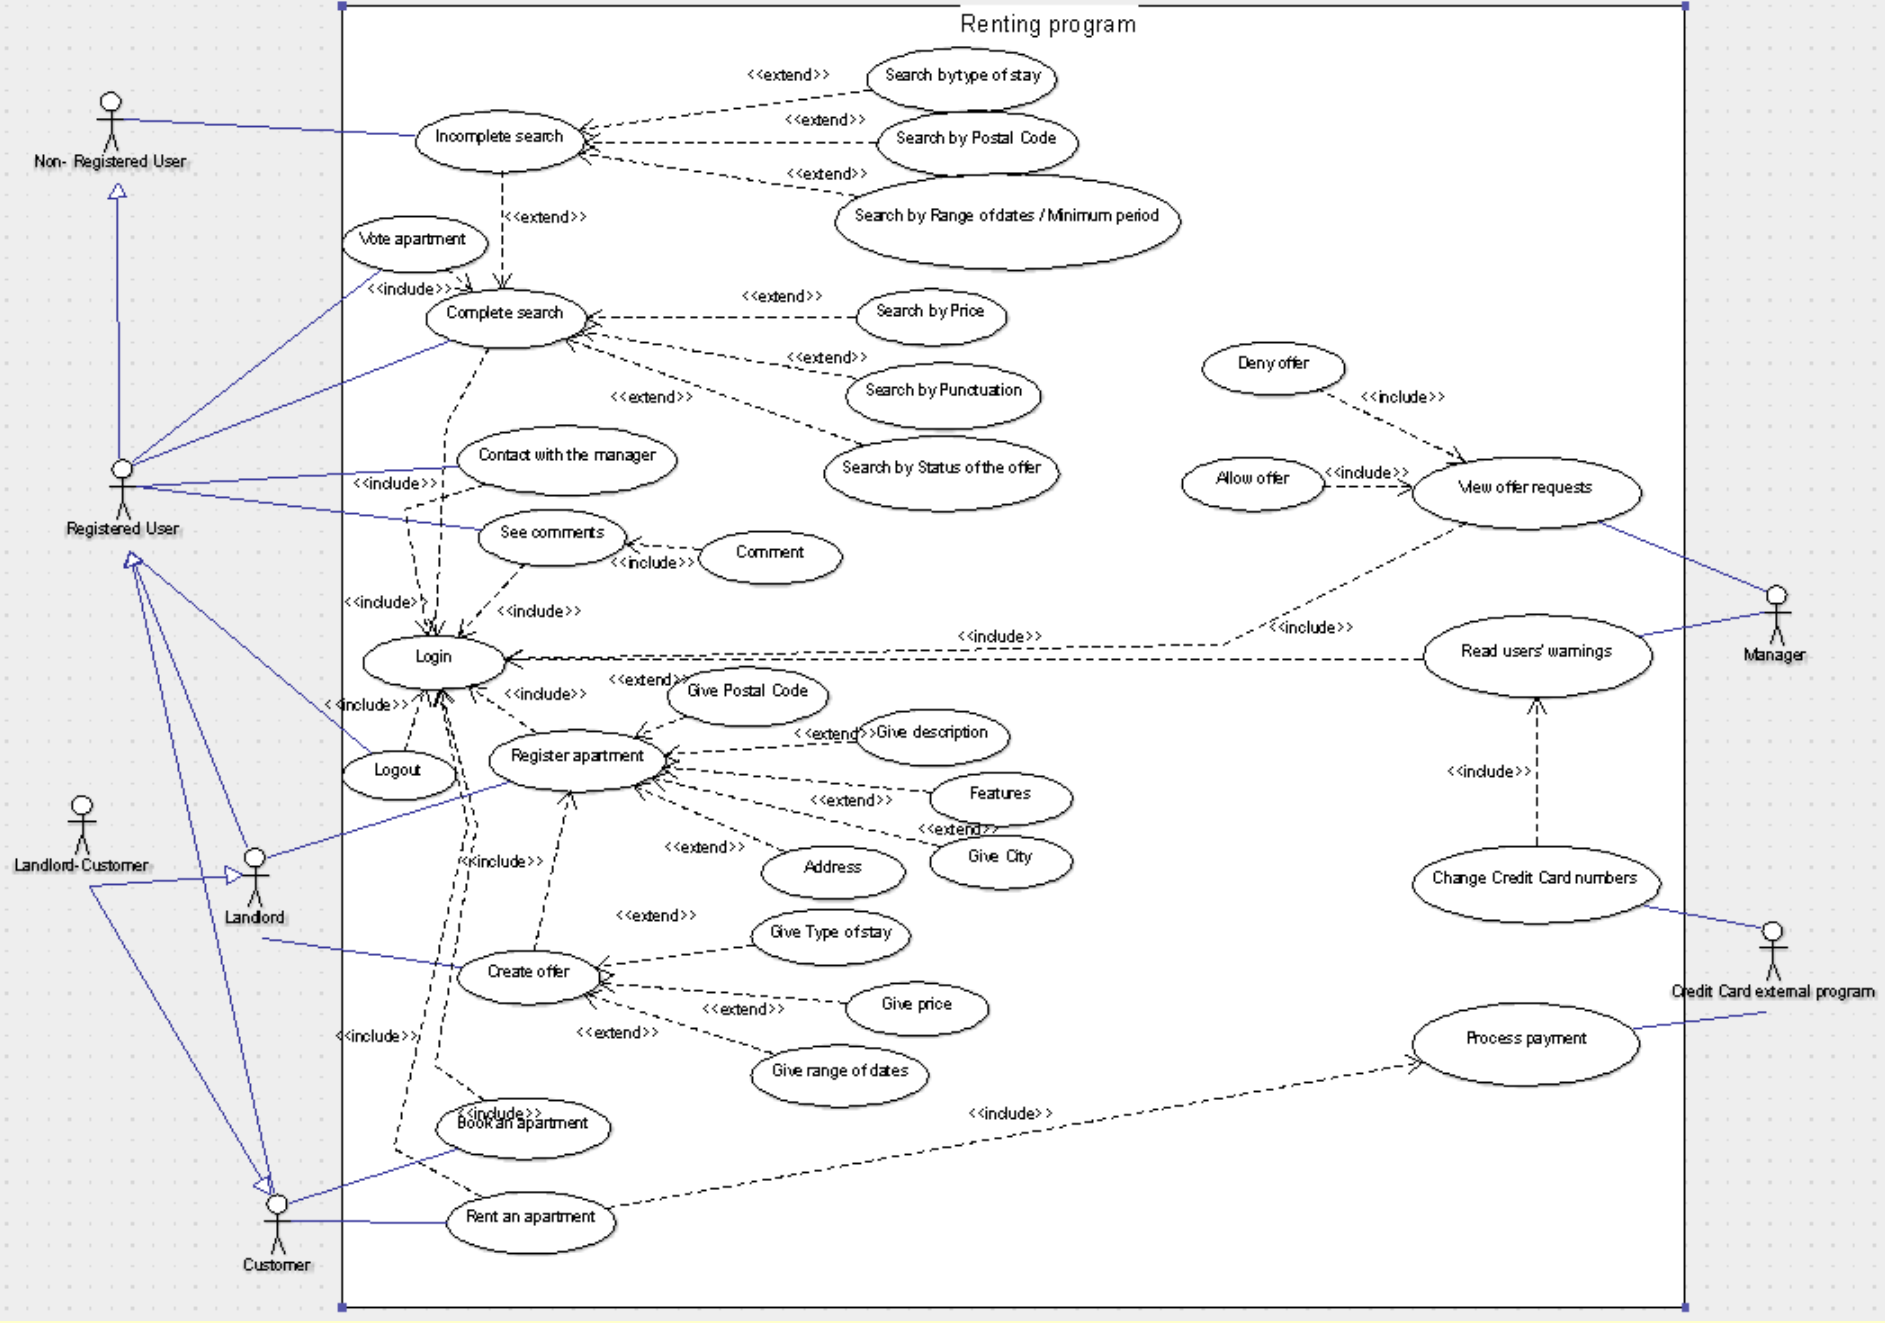
\includegraphics[scale=0.75]{UMLDiagram.PNG}
\end{center}
\subsection{Use Case descriptions}
\subsubsection{Use Case: Register an apartment}
· \underline{Primary Actor:} Landlord and Landlord-Customer.\\\\
· \underline{Stakeholders and Goals:} A premium user registered as Landlord or as a Landlord-Customer has the chance to register one or more properties with the goal of making an offer of them later.\\\\
· \underline{Preconditions:} The user is identified and authenticated as a landlord or as a landlord-customer.\\\\
· \underline{Success guarantee (postconditions):} The whole description (PC, address, features) are written by the user and the system updates the new apartment registration. After that, the property is ready to being offered.\\\\
· \underline{Main Success Scenario:}\\
	1. Landlord or landlord-customer selects "Register property" or "Register apartment".\\
	2. The user enters a full description of the property: PC, address, city and features.\\
	3. The user selects "create" or "apply" (it is versatile) and the system asks if he/she is sure.\\
	4. If the user selects "Yes", the system saves all the information and updates the application.\\\\
· \underline{Extensions (alternative paths):} In point 3, if the user selects "No", the user can still make some changes or even quit the registration.\\\\
· \underline{Special Requirements:} The system has to be able to update in a short period of time when the user presses a key to write. \\\\
· \underline{Technology \& Data Variations List:} None\\\\
· \underline{Frequency:} Really high, in the order of hundeds of users at the same time.\\\\
· \underline{Open Issues:} Autocomplete the city and/or address of the property. It will be usefull to do not allow the registration of nonexistent locations.\\

\subsubsection{Use Case: Create offer}
· \underline{Primary Actor:} Landlord and Landlord-Customer.\\\\
· \underline{Stakeholders and Goals:} A premium user registered as Landlord or as a Landlord-Customer has the chance to make an offer..\\\\
· \underline{Preconditions:} The user is identified and authenticated as a landlord or as a landlord-customer. Moreover, the accommodation that the user wants to offer has to have been previosly registered.\\\\
· \underline{Success guarantee (postconditions):} The whole description (stay type, price, dates) are written by the user. After that, a notification is sent to the manager to approve (or not) the offer.\\\\
· \underline{Main Success Scenario:}\\
	1. Landlord or landlord-customer selects "Create offer".\\
	2. A list of his/her registered properties are shown up.\\
	3. The user selects a property to make an offer.\\
	4. The user writes type of stay, the price and the range of dates(short stay) or the minimum period of renting(long stay).\\
	5. The user selects "Make offer".\\
	6. The system sends a notification to the manager to approve or deny the offer.\\\\
· \underline{Extensions (alternative paths):} In point 2, if the user selects a property to offer, he/she can comeback if he/she has missclicked in the wrong property.\\\\
· \underline{Special Requirements:} The system has to be able to update in a short period of time when the user presses a key to write. \\\\
· \underline{Technology \& Data Variations List:} None.\\\\
· \underline{Frequency:} Really high, in the order of hundeds of users at the same time.\\\\
· \underline{Open Issues:} "Are you sure?" message when the user selects "Make offer" in order to avoid mistakes, but it is not important because the user can modify and edit the offer later (before it is approved).\\

\subsubsection{Use Case: Rent an apartment}
· \underline{Primary Actor:} Customer and Landlord-Customer.\\\\
· \underline{Stakeholders and Goals:} A premium user registered as Customer or as a Landlord-Customer has the chance to rent an apartment..\\\\
· \underline{Preconditions:} The user is identified and authenticated as a customer or as a landlord-customer. In addiction, the status of the accommodation has to be "Free".\\\\
· \underline{Success guarantee (postconditions):} The system, with the external payment application, manages the payment and, if it succeeds, the rent is completed.\\\\
· \underline{Main Success Scenario:}\\
1. Customer or landlord-customer selects an accommodation. He/she might have used the search filter.\\
2. The user is going to examinate the apartment and its features and determine if he/she wants to rent it.\\
3. The user selects "Rent" and the system sends a pop-up asking if he/she is sure.\\
4. If the user selects "Yes", the system manages the payment with the external payment application.\\
5. If the payment succeeds, the apartment is already rented. Then, the system changes apartment's status from "Free" to "Rented".
· \underline{Extensions (alternative paths):} In point 4-5, if the payment fails, the system bans the user. The only thing the user can do is to send a message to the manager in order to change its credit card number.\\\\
· \underline{Special Requirements:} The system has to be able to update in a short period of time when the user presses a key to write. It has to process the payment quite fast as well, due to the fact users are not patient.\\\\
· \underline{Technology \& Data Variations List:} None.\\\\
· \underline{Frequency:} Quite high, in the order of thousands of concurrent users.\\\\
· \underline{Open Issues:} Working on a good message or alternative way to improve the banning system if the credit card fails to pay.\\

\subsubsection{Use Case: Comment}
· \underline{Primary Actor:} Any registered user: landlord, customer or landlord-customer.\\\\
· \underline{Stakeholders and Goals:} A registered user can comment on the apartments description page, in order to advice other people if their experience has been gratifying or not. Moreover, the comments can be used to try to contact with the owner of the property and ask something.\\\\
· \underline{Preconditions:} The user is identified and authenticated, and has sought an accommodation.\\\\
· \underline{Success guarantee (postconditions):} The whole comment is written and ready to be posted.\\\\
· \underline{Main Success Scenario:}\\
1. Registered users selects any offer.\\
2. The user writes a comment on the comments section of the page.\\
3. The user selects "send" or "confirm" (it is versatile).\\
4. The system saves the comment and updates the information.\\\\
· \underline{Extensions (alternative paths):} Once you decide to comment, there is no alternative path.\\\\
· \underline{Special Requirements:} The system has to be able to update in a short period of time when the user presses a key to write.\\\\
· \underline{Technology \& Data Variations List:} None.\\\\
· \underline{Frequency:} Very high, in the order of thousands of concurrent comments.\\\\
· \underline{Open Issues:} Corrector that automatically checks and improves writting.\\\\


\section{Mockups}
· \underline{1.-Principal page (short):} Showing the principal page, where you are browsing as a public user and you can only search by type of stay (short stay is marked), postal code and range of dates, becuase of the fact short stay is selected. Loging in at \textcolor{red}{(1)} will send you to mockup number 3 or mockup number 12, depeding on the type of the user. 
\begin{center}
	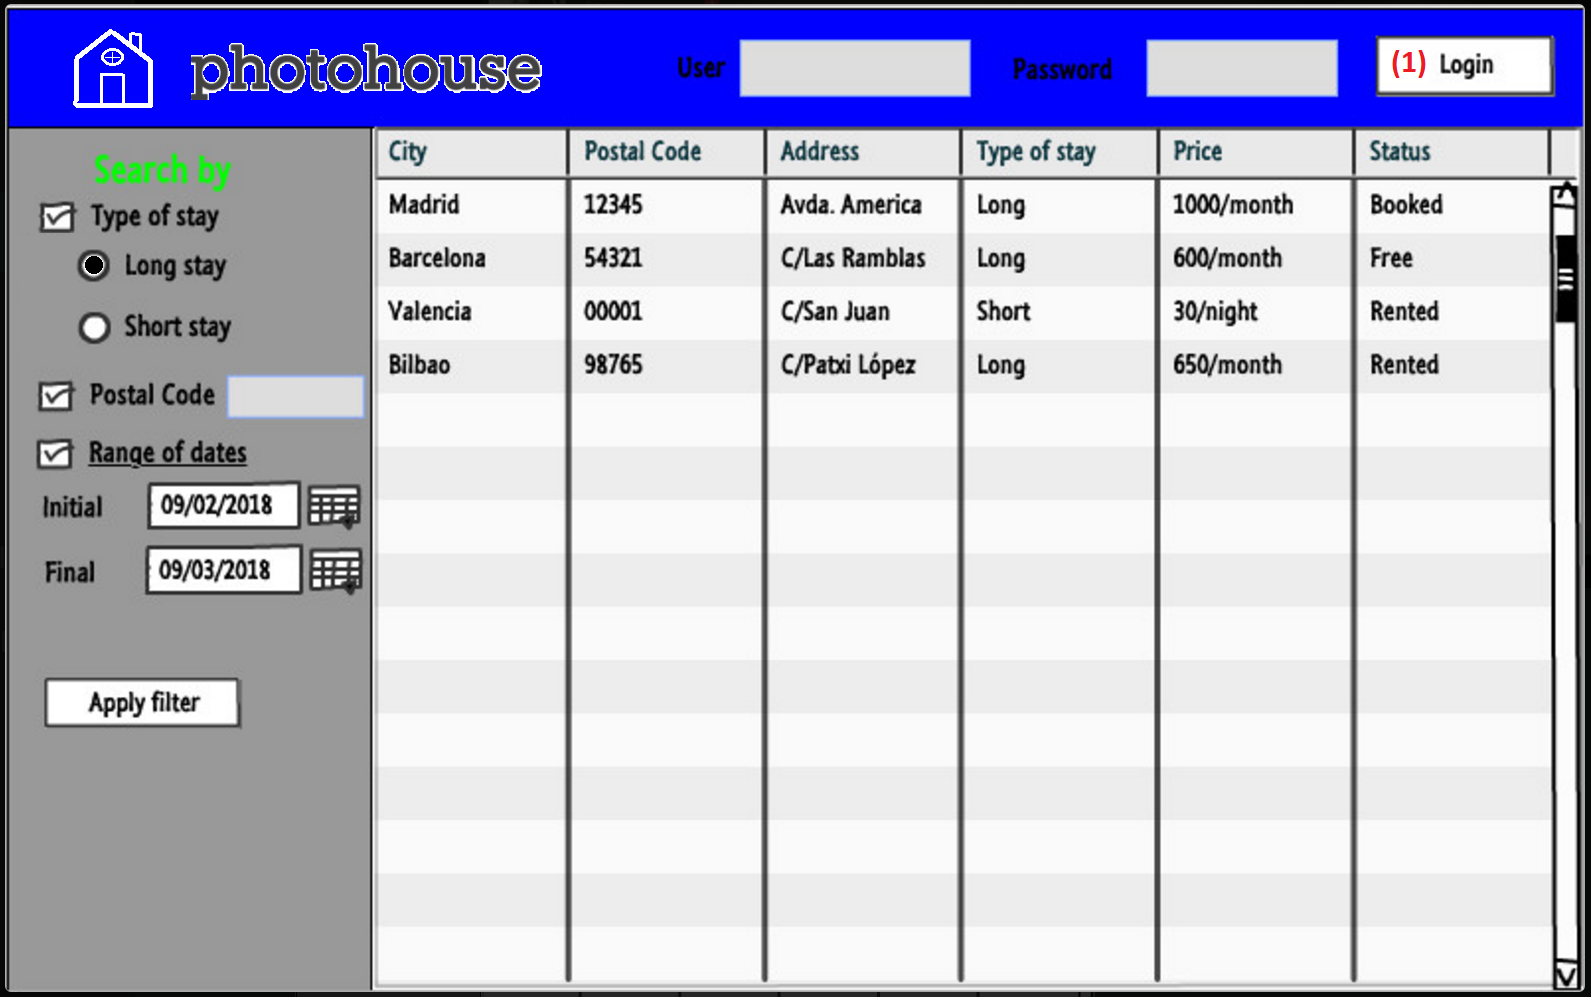
\includegraphics[scale=.7]{principal_short.PNG}
\end{center}

\newpage
· \underline{2.-Principal page (long):} Browsing as a public user in the principal page. You can only search by type of stay (long stay is marked), postal code and minimum period, due to the fact short stay is selected. 
\begin{center}
	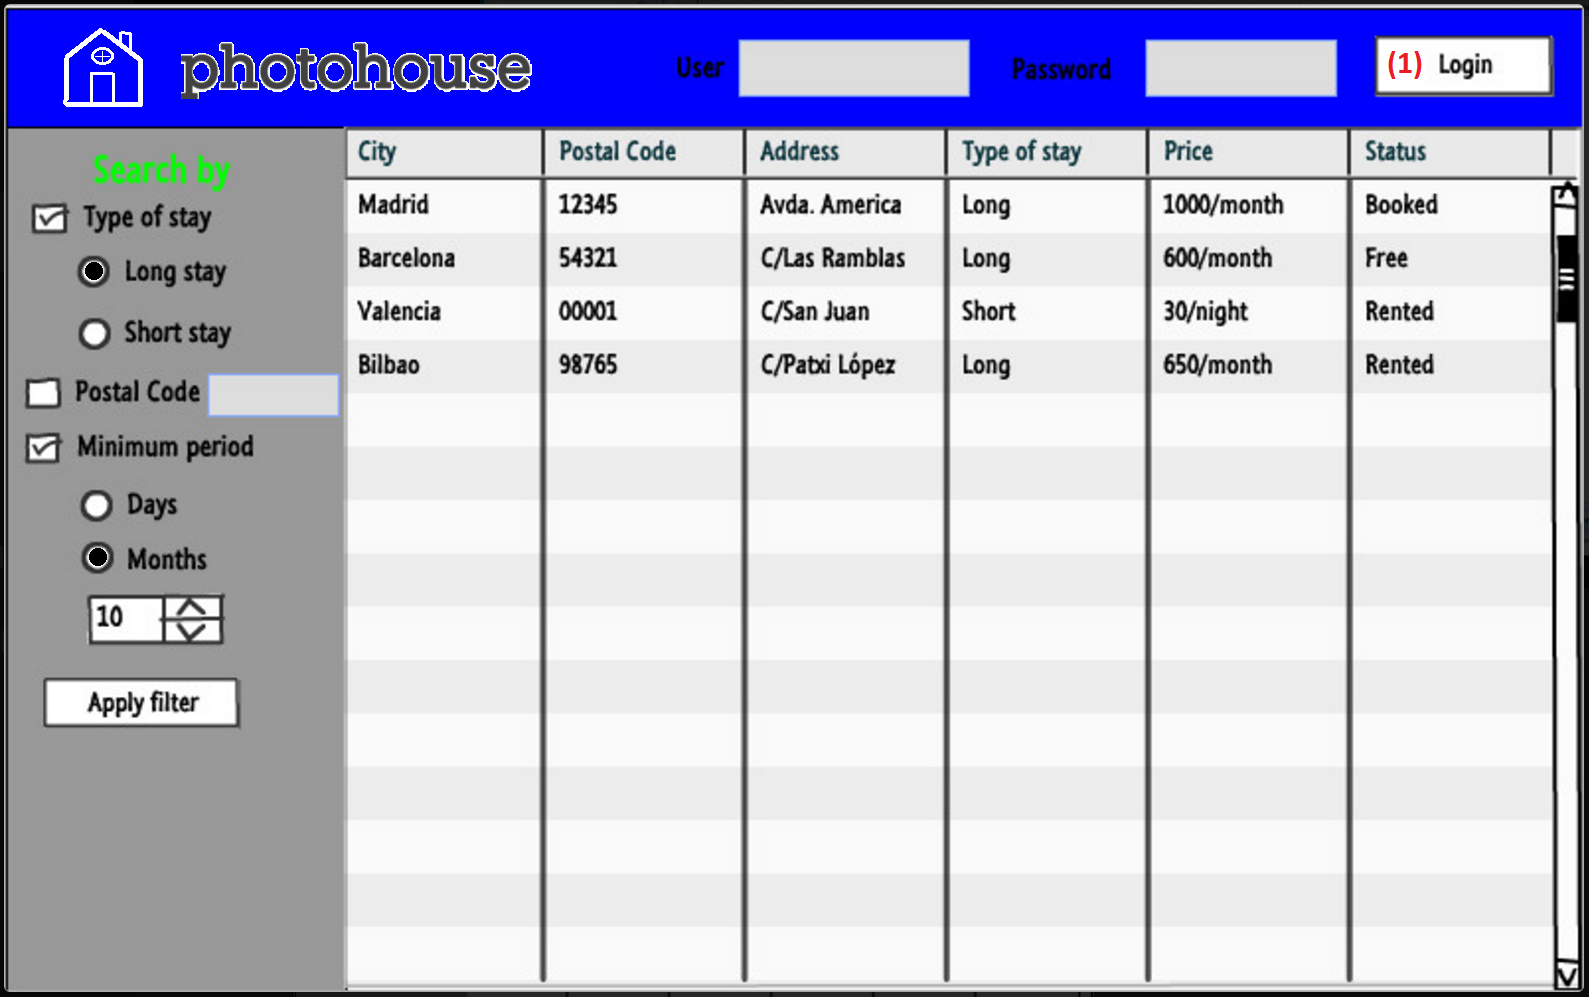
\includegraphics[scale=.7]{principal_long.PNG}
\end{center}


· \underline{3.-Landlord Principal page:} You are registered as a landlord at this moment. We are going to explain what you can do.\\ Pressing at \textcolor{red}{(2)} to see an offer (mockup number 4), but you can't rent it if you are only a Landlord.\\ Click on \textcolor{red}{(3)} to see your registered properties (mockup number 5); and select \textcolor{red}{(4)} to check your offers (mockup number 6).\\ You can register a new property by pressing \textcolor{red}{(5)} (mockup number 7); and you can create an offer of a registered property by selecting \textcolor{red}{(6)} (mockup number 8).\\ You can also send a message to the manager in order to change your credit card number by pressing \textcolor{red}{(7)} (mockup number 17).\\ One really important part of this page is to keep in mind you can search by a lot of things as a registered user that public users can't, just take a look at the left panel \textcolor{red}{(*)}.Finally, you can log out with the buttom "Log out" \textcolor{red}{(8)} that will drive you to mockup number 1 or 2.
\begin{center}
	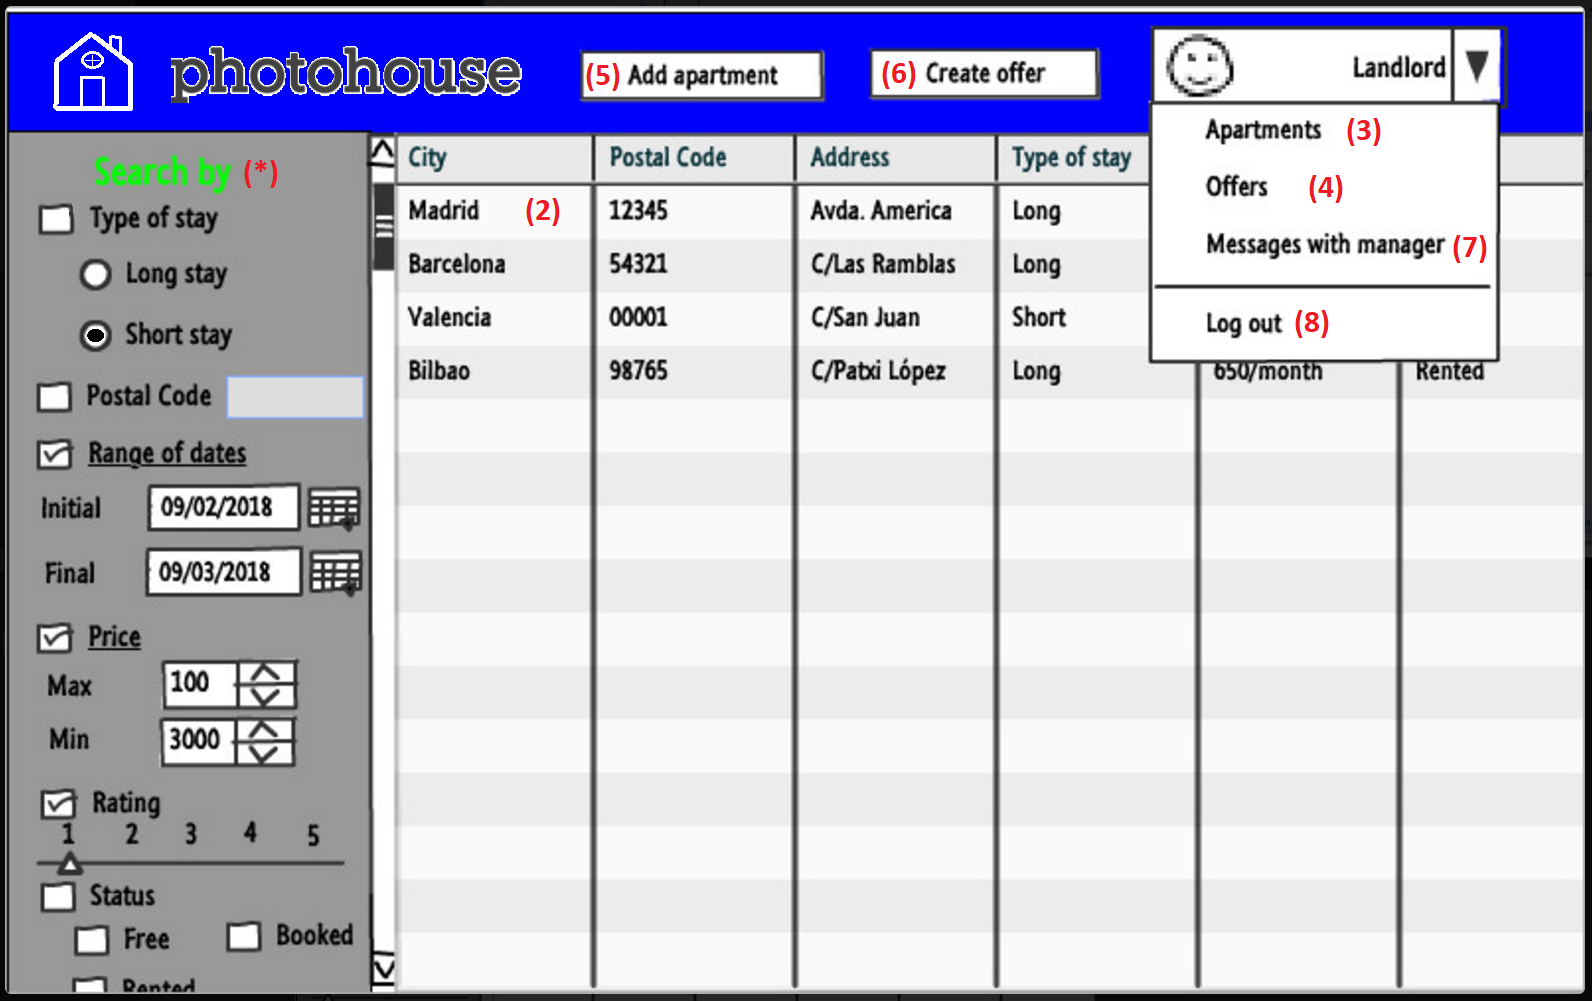
\includegraphics[scale=.7]{landlord.PNG}
\end{center}


· \underline{4.-Landlord trying to rent:} You cannot rent an accommodation as a Landlord as the left message indicates. However, you can see comments, vote an apartment choosing a mark and voting \textcolor{red}{(9)}; and even commenting in the comments section \textcolor{red}{(10)}.You can comeback to the previous view clicking on \textcolor{red}{(11)}.\\
\begin{center}
	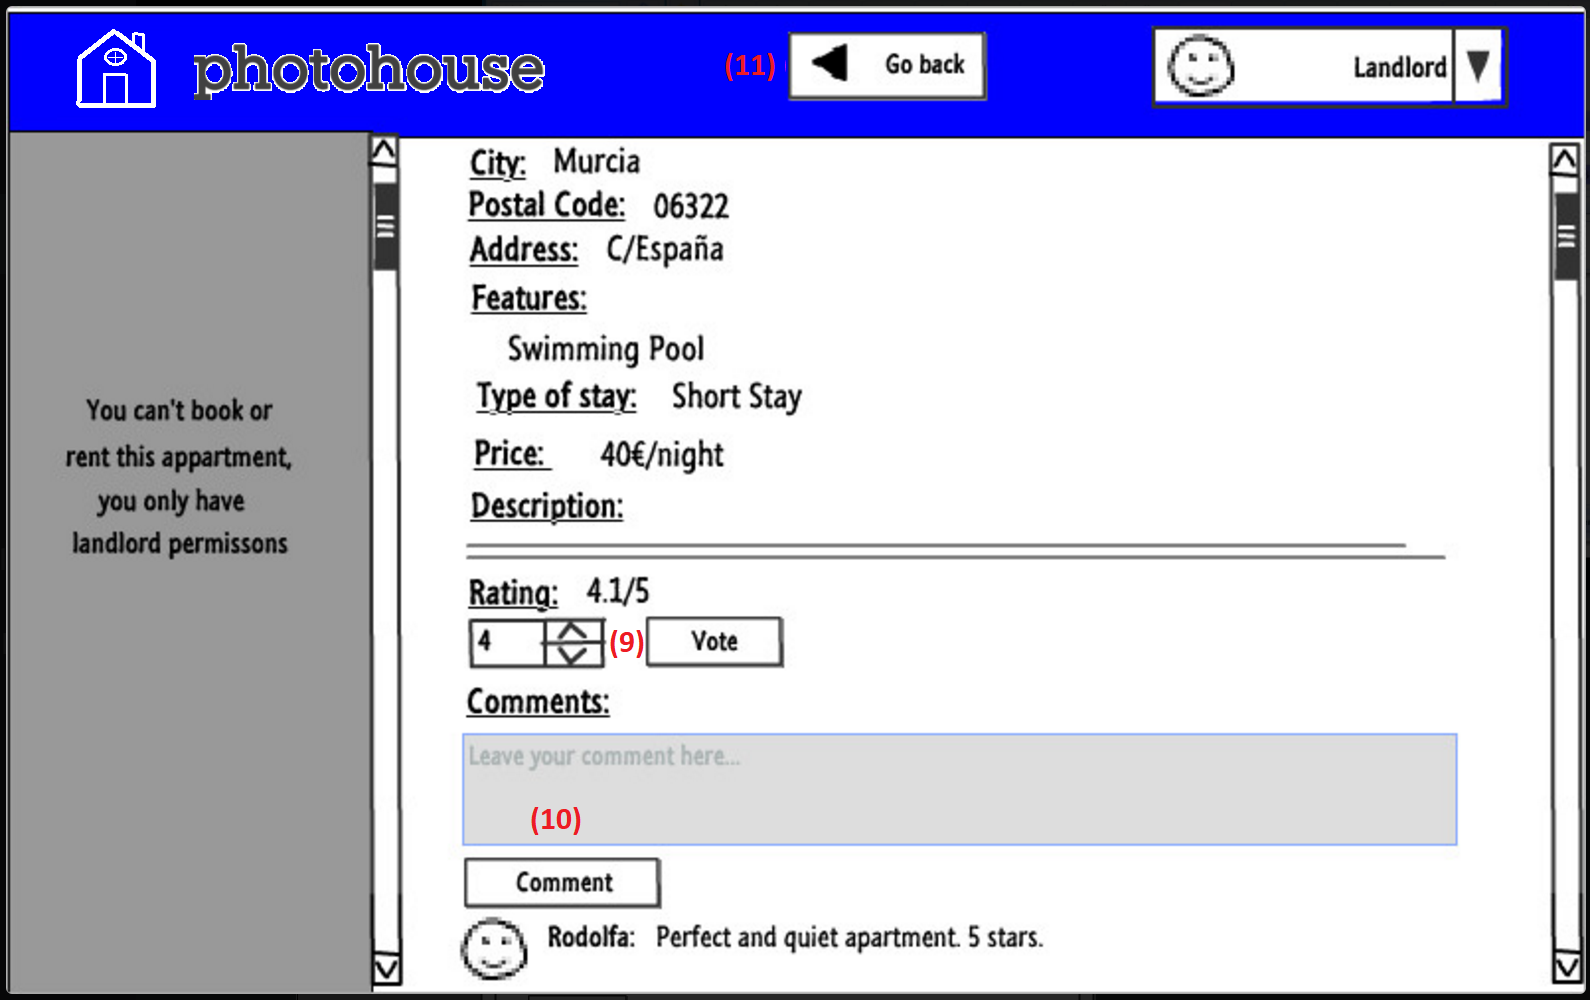
\includegraphics[scale=.7]{landlord_renting.PNG}
\end{center}

\newpage
· \underline{5.-Landlord checking its properties:} Landlords can watch its properties by just cliking on the top lash \textcolor{red}{(12)}.
\begin{center}
	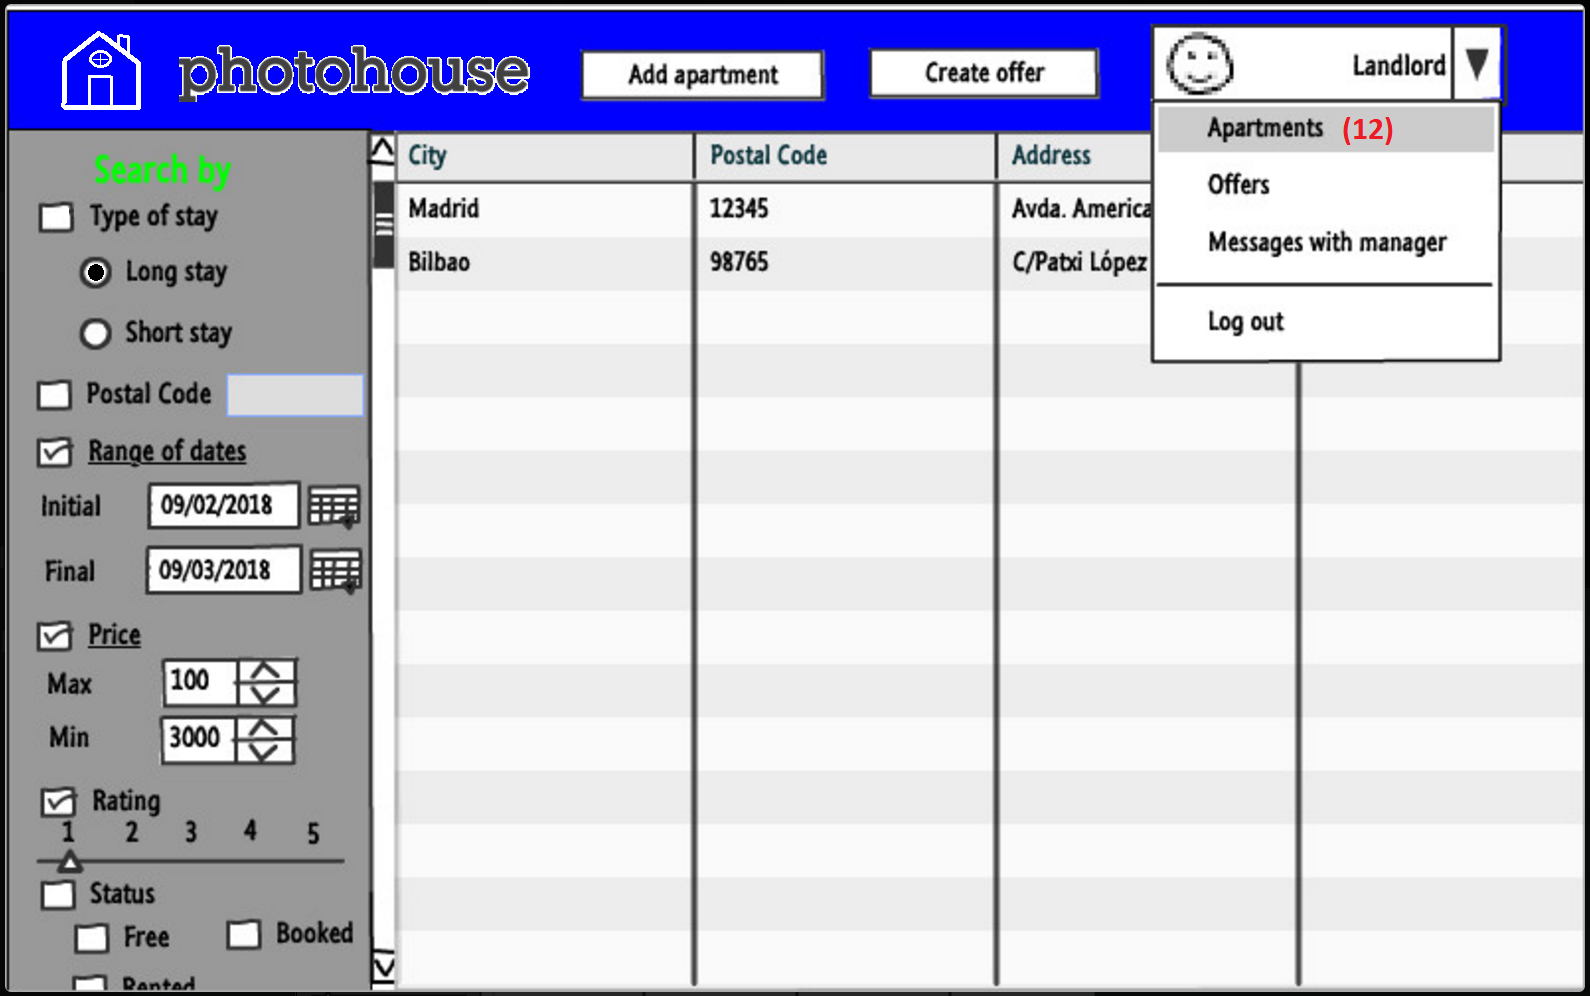
\includegraphics[scale=.7]{landlord_apartments.PNG}
\end{center}


· \underline{6.-Landlord checking its offers:} Doing barely the same, Landlords can check its offers \textcolor{red}{(13)}.
\begin{center}
	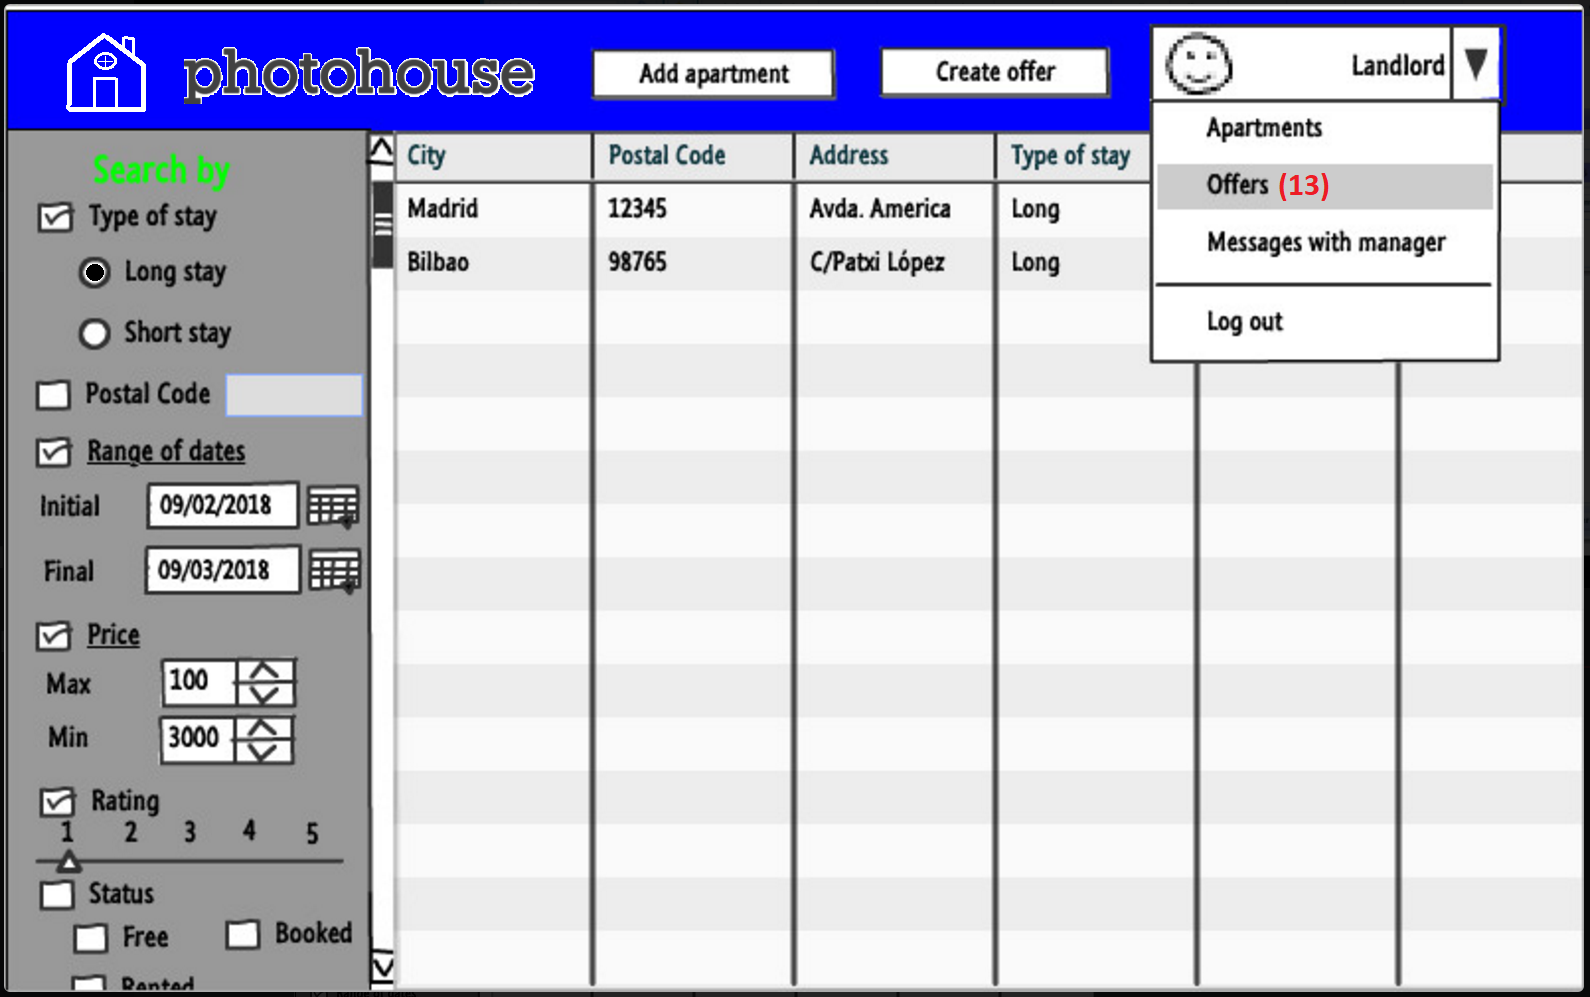
\includegraphics[scale=.7]{landlord_offers.PNG}
\end{center}

\newpage
· \underline{7.-Landlord registering a property:} As we said, we are now in the properties registration page, where the landlord is supossed to add an apartment.\\ We can write the city \textcolor{red}{(14)}, the Postal Code \textcolor{red}{(15)}, the address \textcolor{red}{(16)} and add some features \textcolor{red}{(17)}, including comments of the apartment \textcolor{red}{(18)}.\\ When you finish you can cancel de registration \textcolor{red}{(20)}, or add the apartment\textcolor{red}{(19)} (a popup message is supossed to apear asking if you are sure to add, but we didn't include it for simplicity).
\begin{center}
	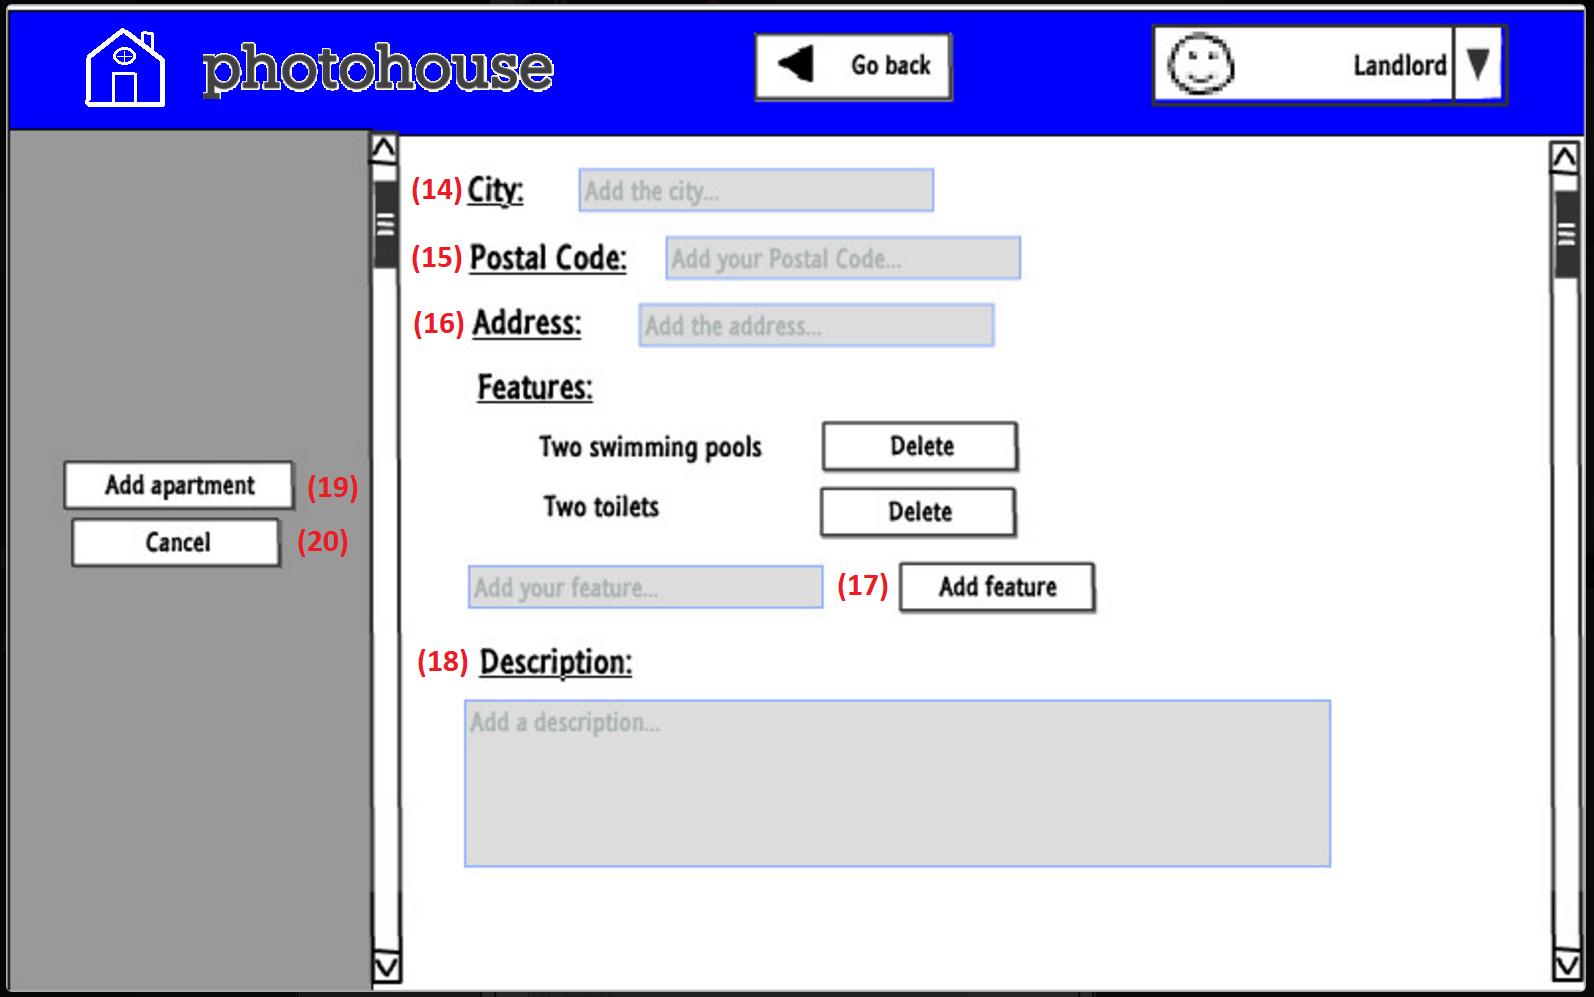
\includegraphics[scale=.7]{landlord_registering.PNG}
\end{center}


· \underline{8.-Landlord making an offer:} Now we are showing how to offer a property. We can choose the apartment to offer from a list of registered apartments \textcolor{red}{(21)}, select the type of stay \textcolor{red}{(22)}, put the price \textcolor{red}{(23)} and indicate the range of dates or the minimum period\textcolor{red}{(24)} (in this example long period is selected but we have already seen how it would be with short stay).\\ When it is finished, you can cancel the offer \textcolor{red}{(26)}, or create the offer\textcolor{red}{(25)} (a popup message is supossed to apear asking if you are sure to create, but we didn't include it for simplicity).
\begin{center}
	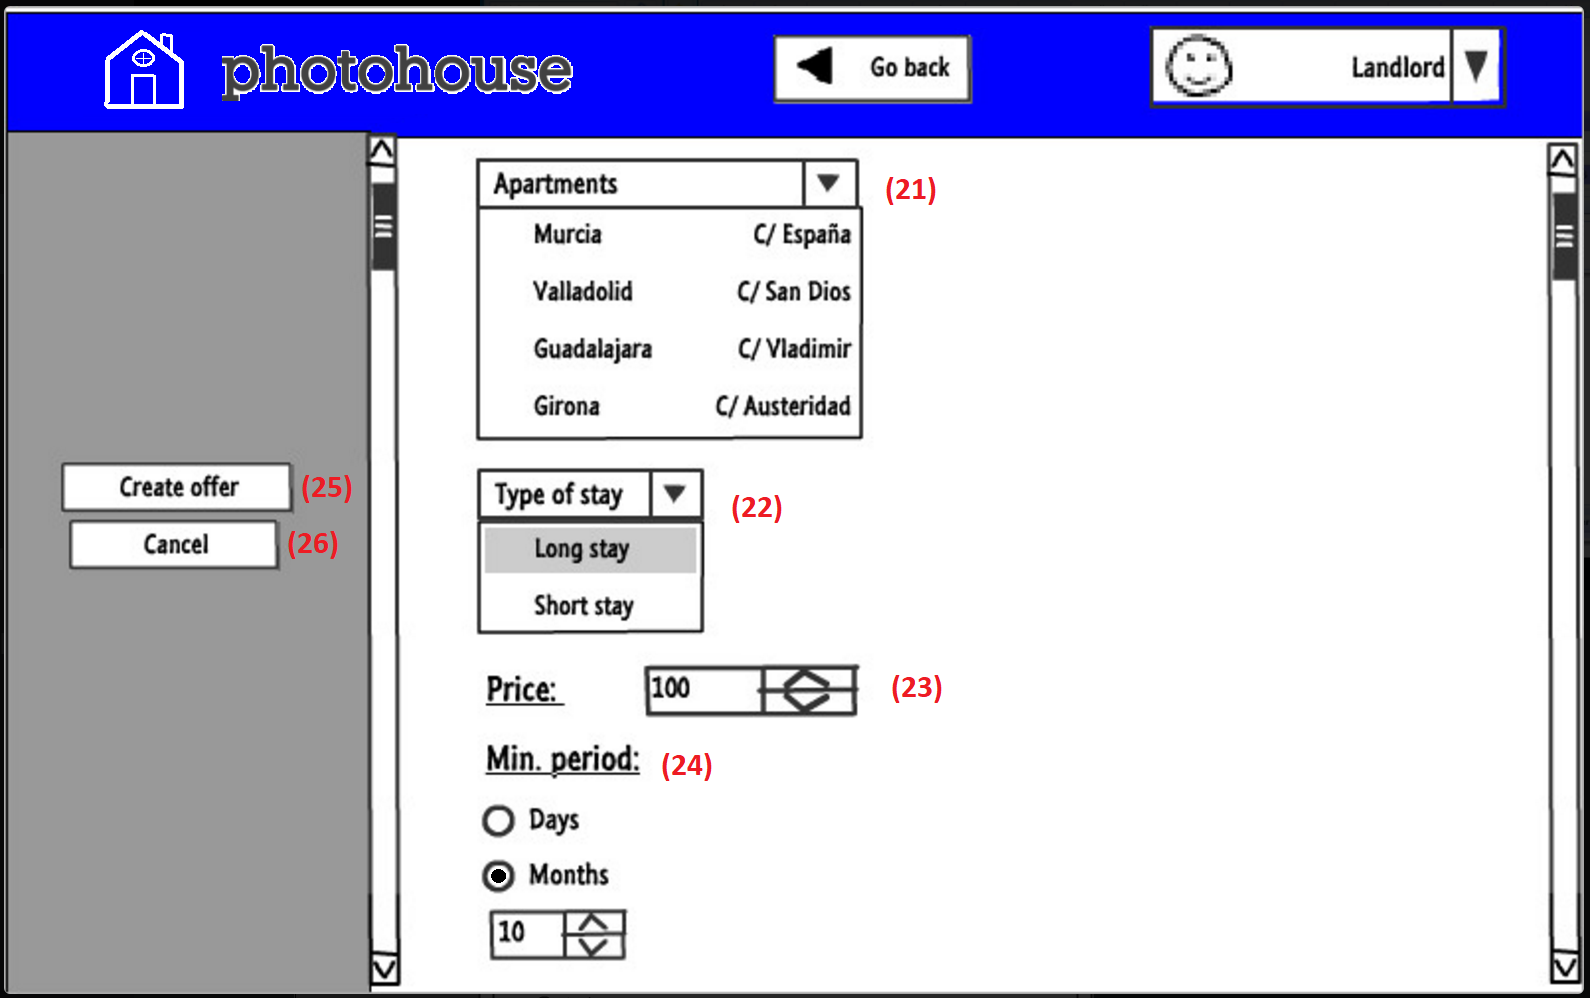
\includegraphics[scale=.7]{landlord_offering.PNG}
\end{center}


· \underline{9.-Landlord modifying an offer part 1:} Landlords can edit its offers before they get approved, pressing \textcolor{red}{(27)}.
\begin{center}
	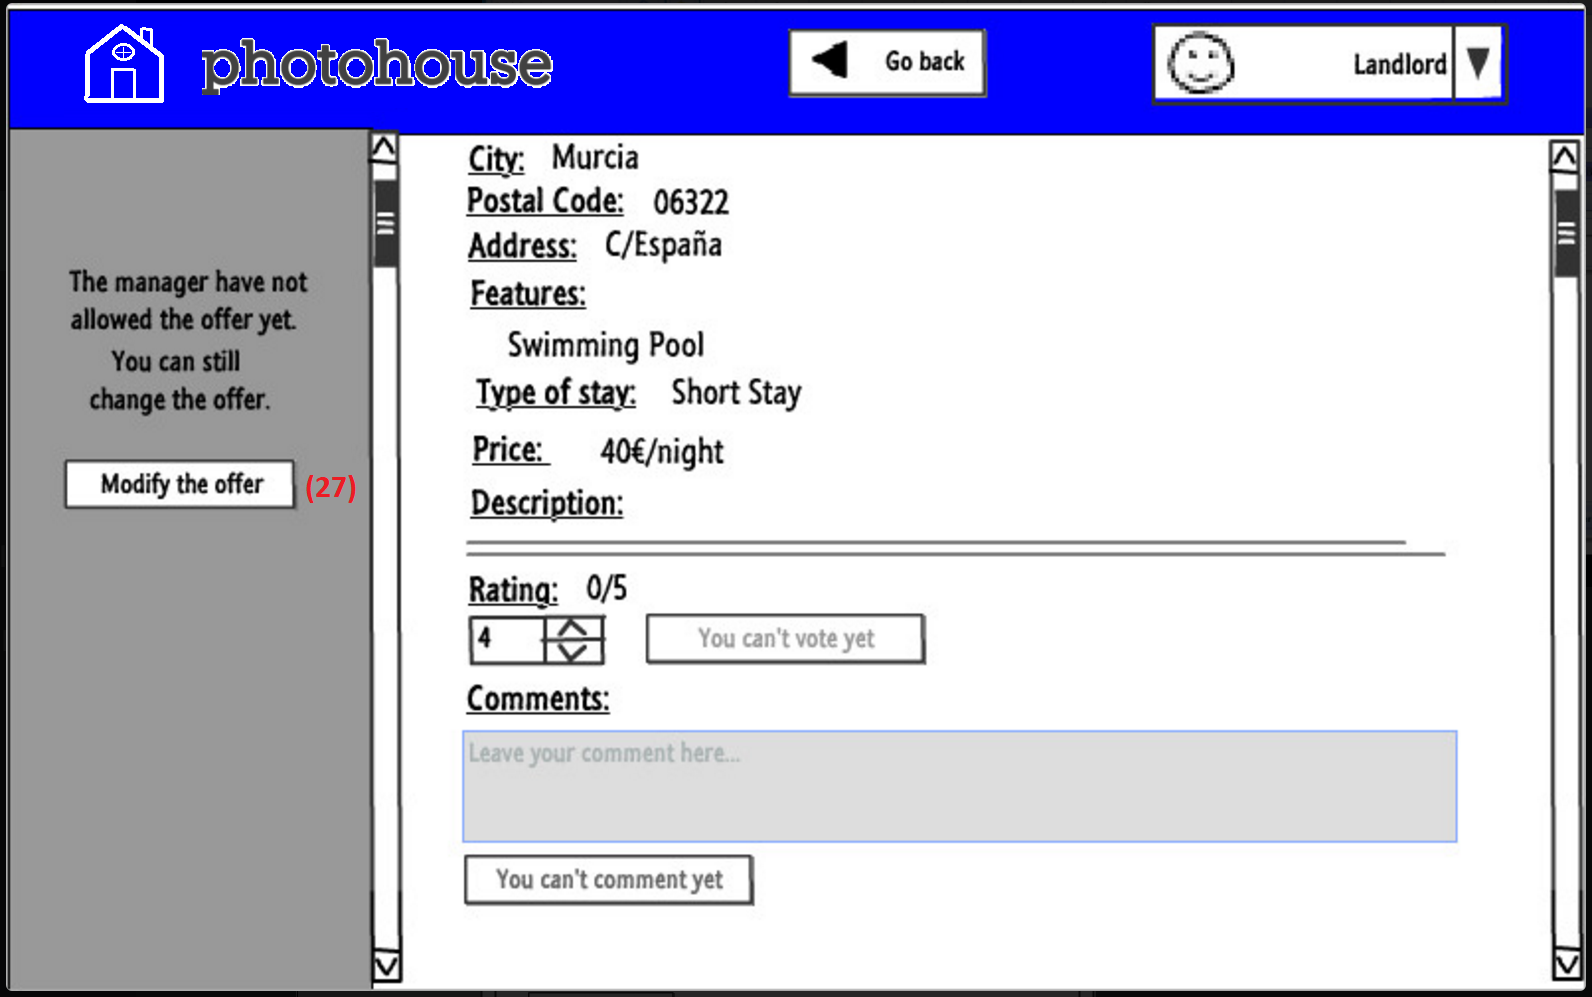
\includegraphics[scale=.7]{landlord_editing.PNG}
\end{center}


· \underline{10.-Landlord modifying an offer part 2:} This mockup is very similar to the 8th one, but now we are not creating an offer, we are editing it. You can change all the shown fields, and pressing cancel or save the changes \textcolor{red}{(28)}.
\begin{center}
	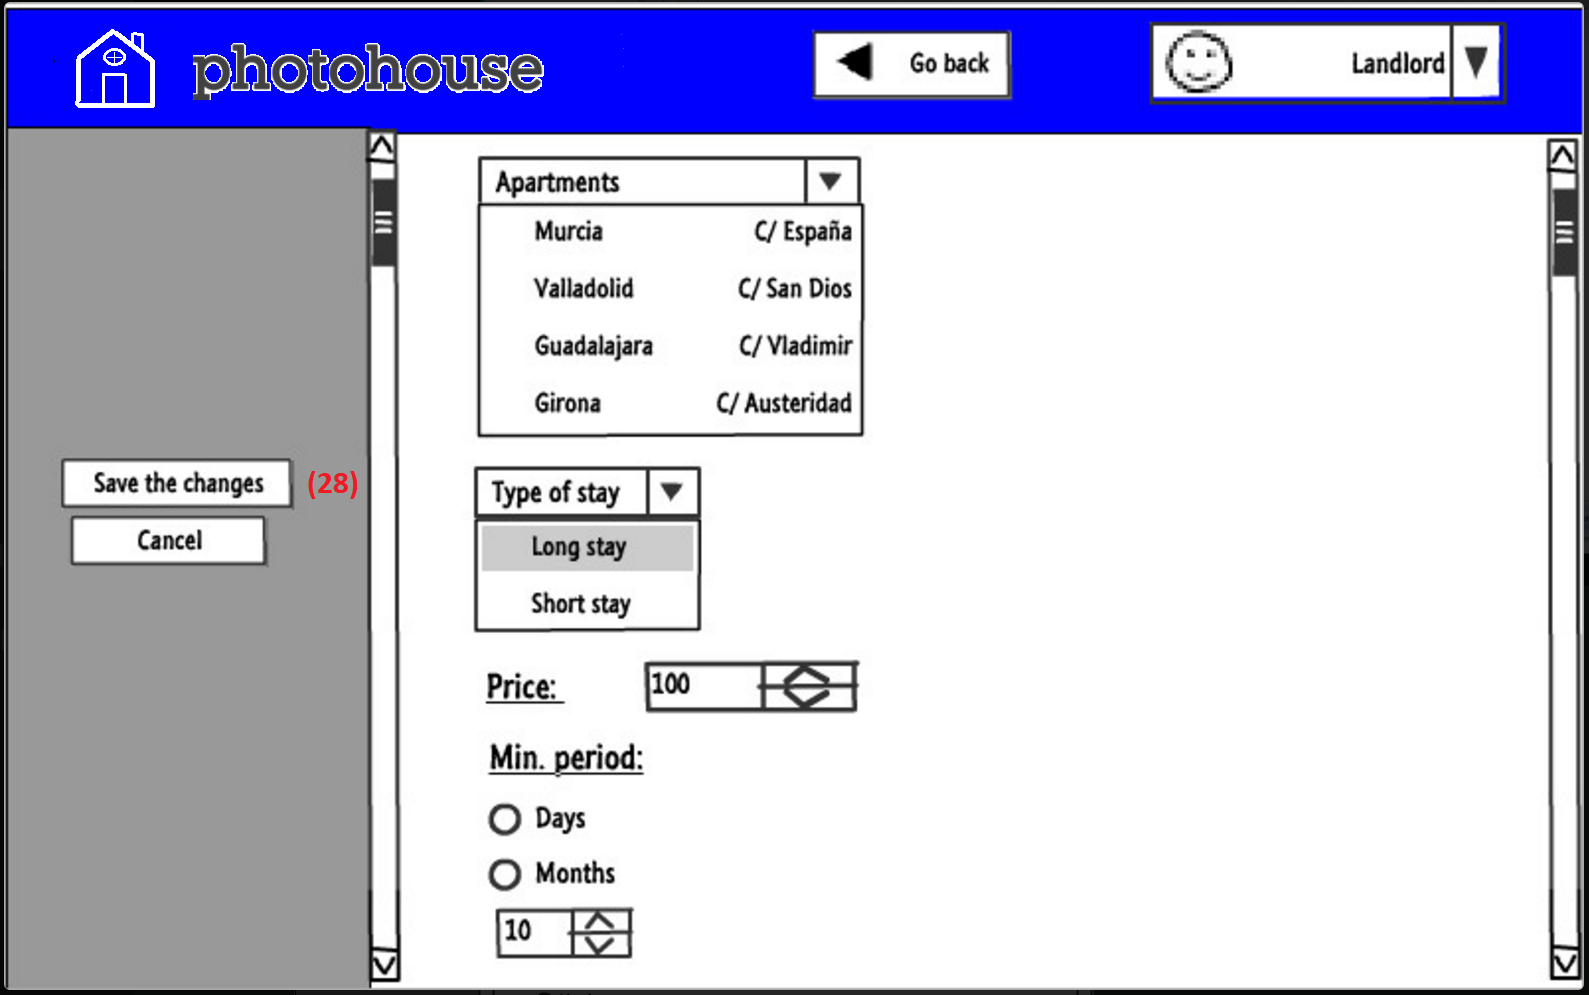
\includegraphics[scale=.7]{landlord_editing_allowed.PNG}
\end{center}


· \underline{11.-Landlord modifying an offer part 3:} That is what PhotoHouse would show if we try to modify an offer that is approved.
\begin{center}
	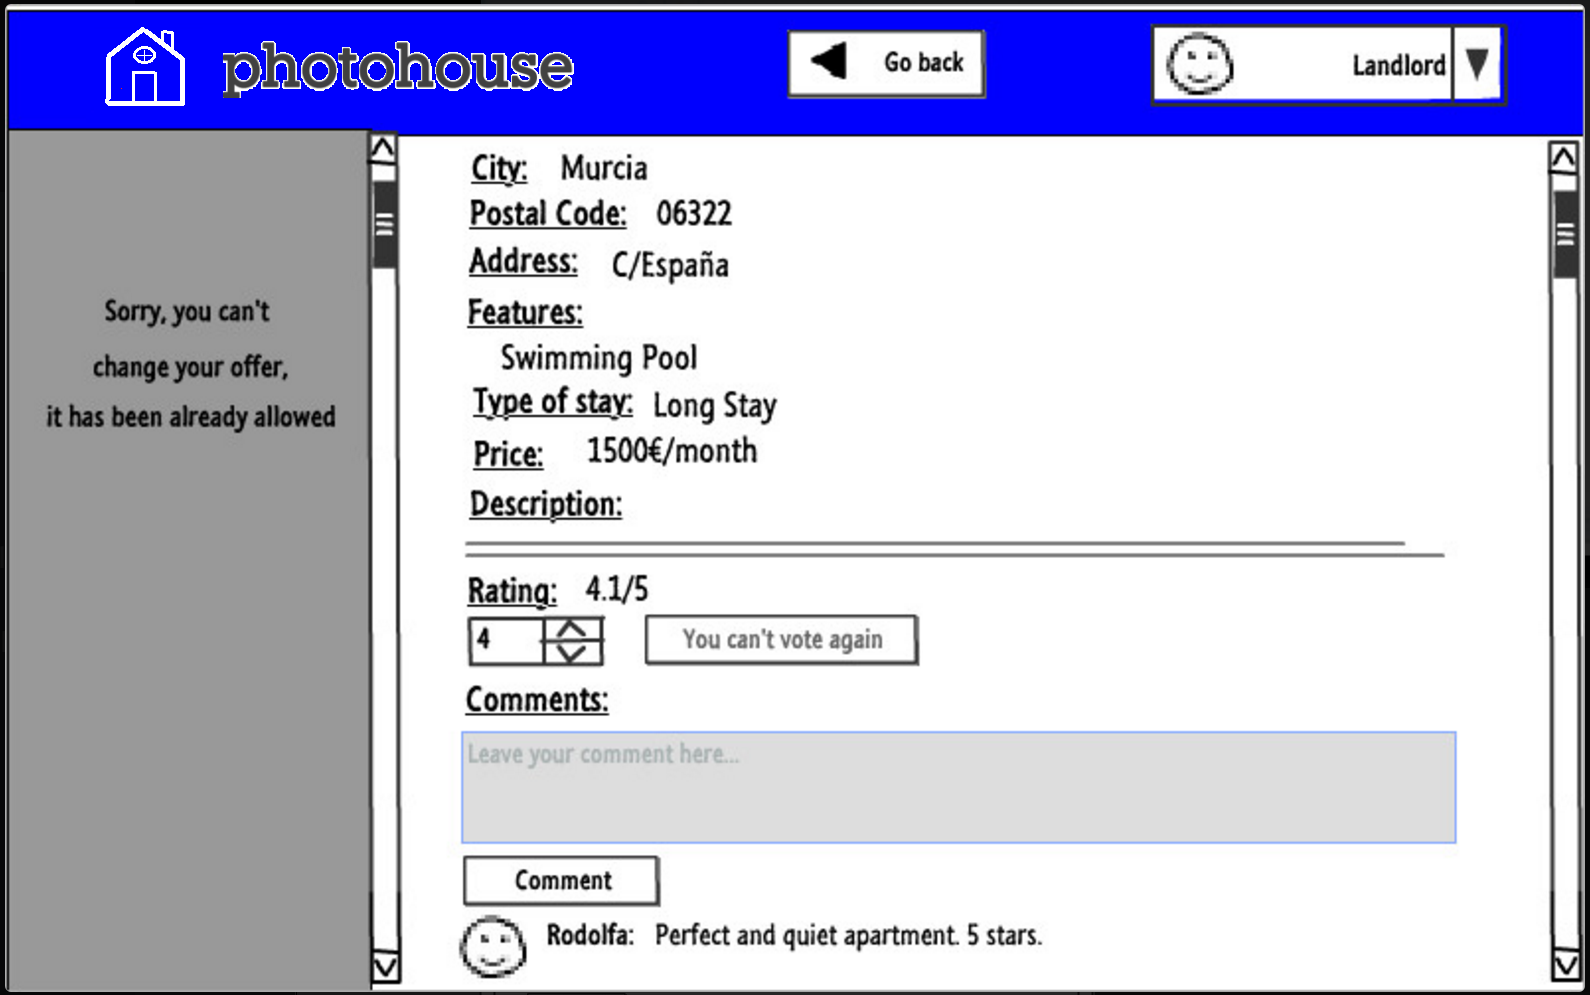
\includegraphics[scale=.7]{landlord_editing_denied.PNG}
\end{center}


· \underline{12.-Customer Principal page:} Most of the options are already explained because are the same than the landlords options. But we got new actions too. First, we can check our rented apartments \textcolor{red}{(29)} (mockup number 13), because now we are able to rent accommodations. Moreover, we can book apartments \textcolor{red}{(30)} (mockup number 14) to think twice what to do. As we told before, press \textcolor{red}{(31)} to change your credit card number by talking with the manager (mockup 17).
\begin{center}
	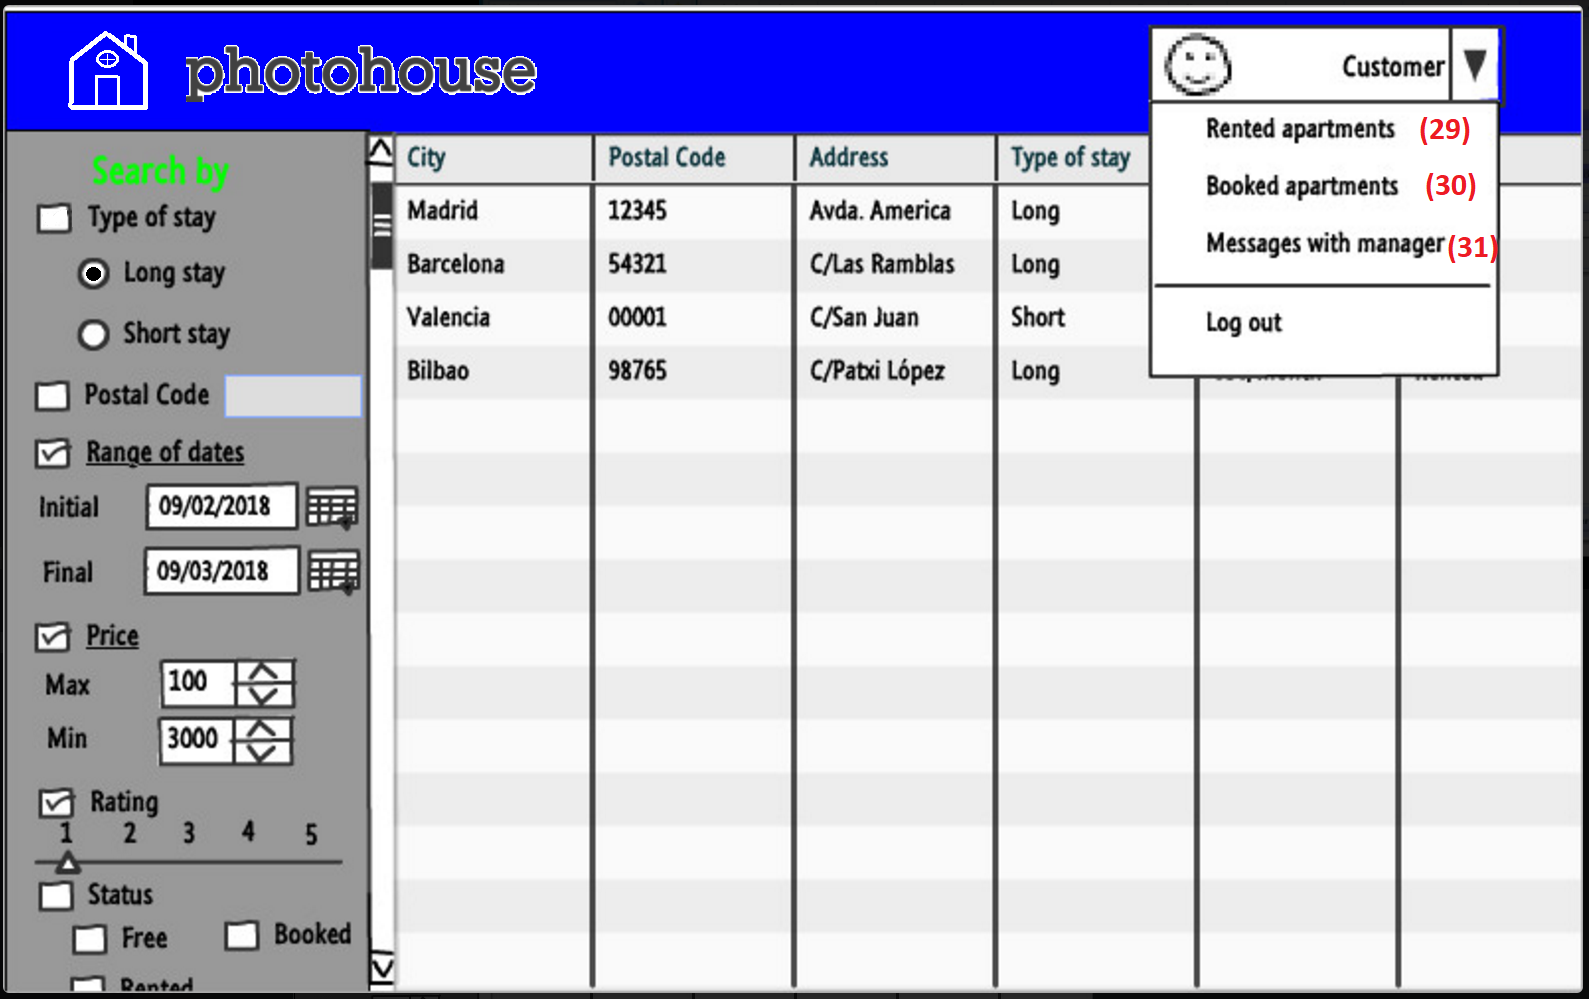
\includegraphics[scale=.7]{customer.PNG}
\end{center}


· \underline{13.-Customer checking its rented properties:} Customers can watch its rented properties by just cliking on the top lash \textcolor{red}{(32)}.
\begin{center}
	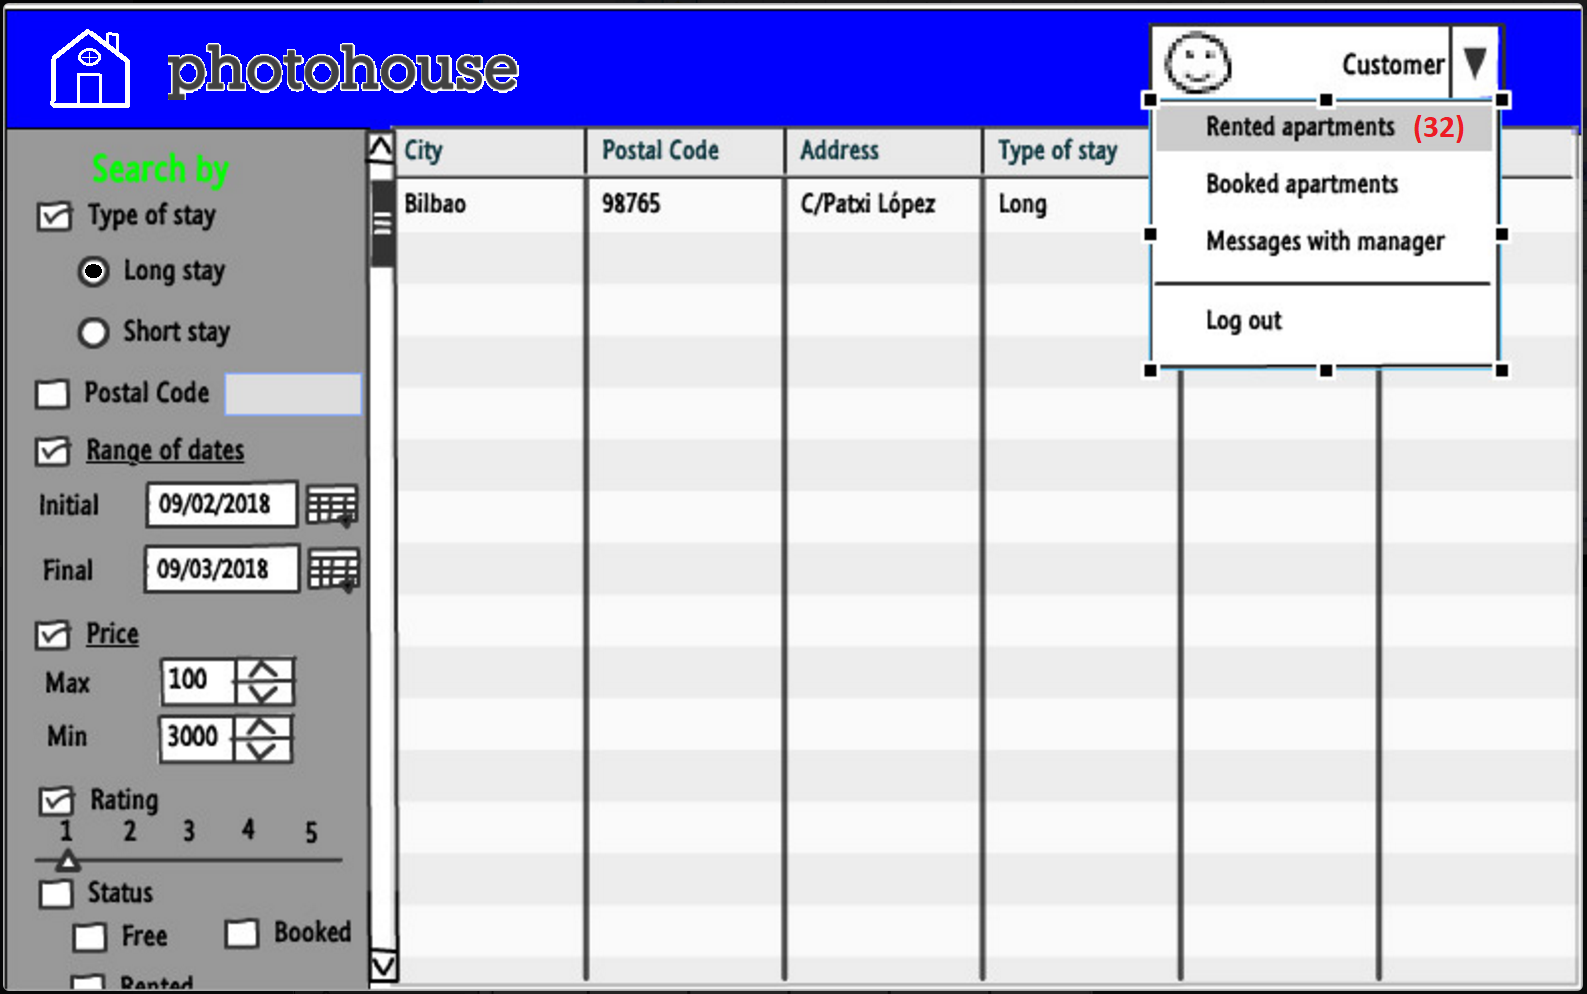
\includegraphics[scale=.7]{customer_rented.PNG}
\end{center}

\newpage
· \underline{14.-Customer checking its reservations:} Doing barely the same, Customers can check its bookings \textcolor{red}{(33)}.
\begin{center}
	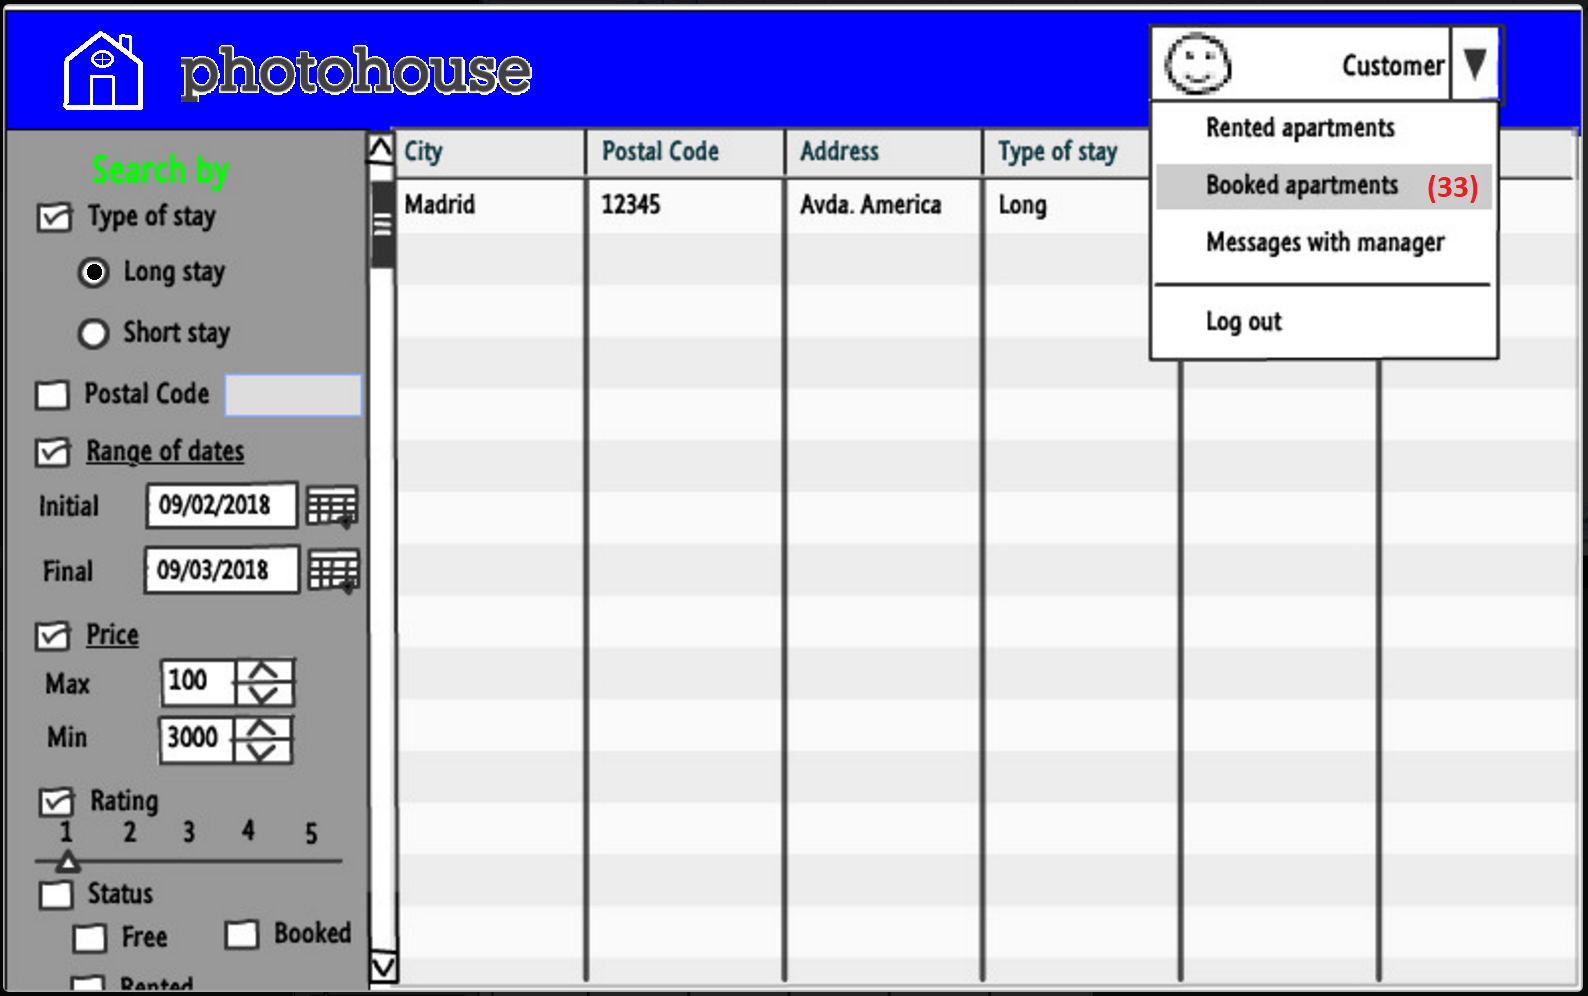
\includegraphics[scale=.7]{customer_booked.PNG}
\end{center}


· \underline{15.-Customer renting part 1:} Customers can rent an accommodation cliking one of the list and the screen will show this mockup. This is a short stay type, so the initial date and the final date of the stay are shown. You can book the property for 5 days \textcolor{red}{(34)} or rent it\textcolor{red}{(35)} (keep in mind that a popup message will appear in order to confirm you want to rent it). You can also comment \textcolor{red}{(36)} or give a puntuation \textcolor{red}{(37)} to the apartment.
\begin{center}
	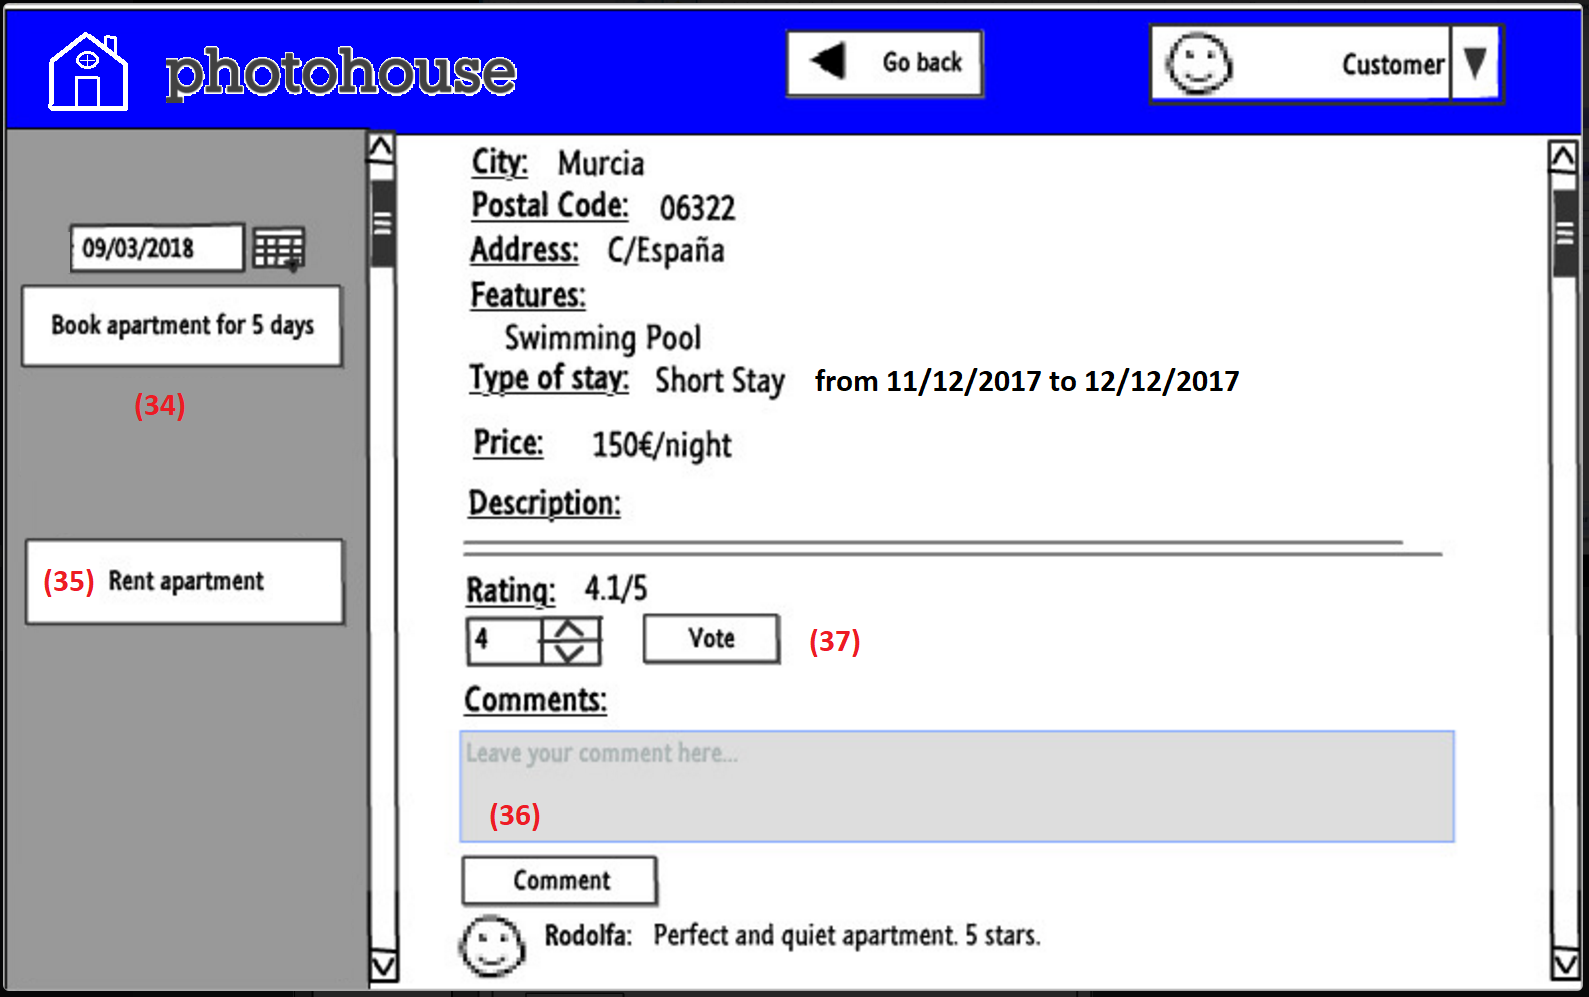
\includegraphics[scale=.7]{customer_renting_short.PNG}
\end{center}

\newpage
· \underline{16.-Customer renting part 2:} It is almost the same one than the one before, but now it is a long stay type, so the minimum period is shown.
\begin{center}
	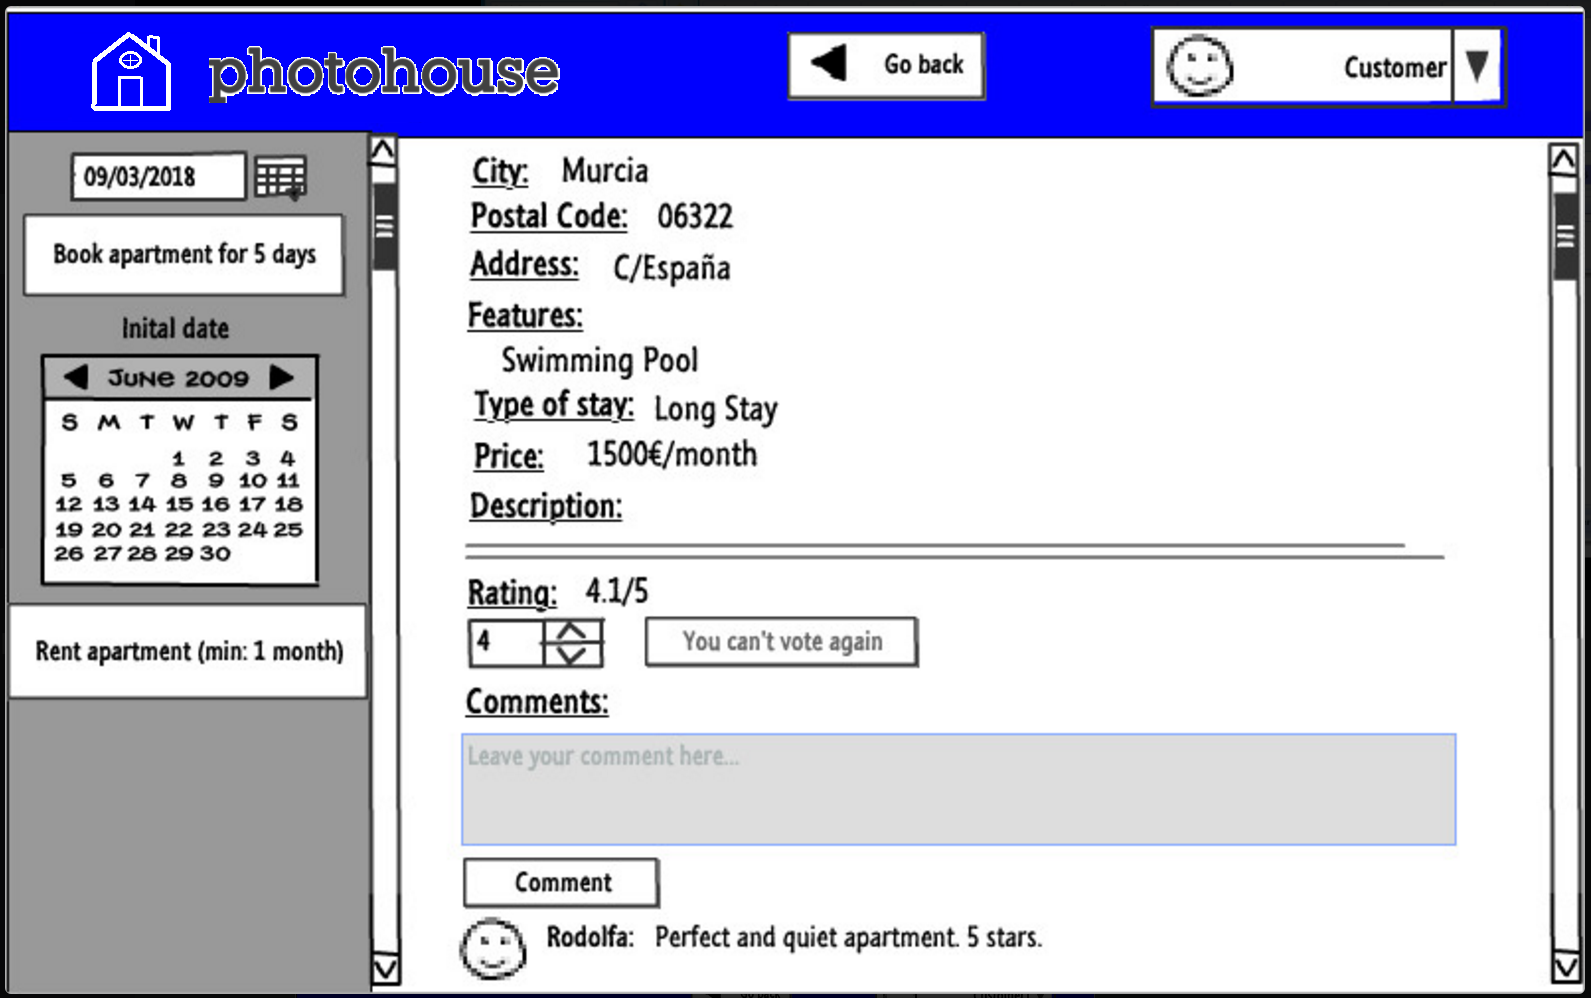
\includegraphics[scale=.7]{customer_renting_long.PNG}
\end{center}


· \underline{17.-Customer-Landlord changing its credit card number:} Here we come if we try to change our credit card number. First, you can check the number in \textcolor{red}{(38)}. If it has expired,\textcolor{red}{(39)} this message will appear. Finally, if you want to contact with the manager, send him the new credit card number at \textcolor{red}{(40)}.\\In this case, the user is not blocked because he is also a Landlord, who do not get banned if their credit card expires. However, if the registered user is only a Customer, he gets banned instantly and he is getting unbanned as soon as he/she changes its credit card number. Check it at mockup number 18.\\
NOTE: Keep in mind that there are registered users as Customers-landlords, we have not shown anything about them, but they have the same permits than the customers plus all of the landlords \textcolor{red}{(41)}.
\begin{center}
	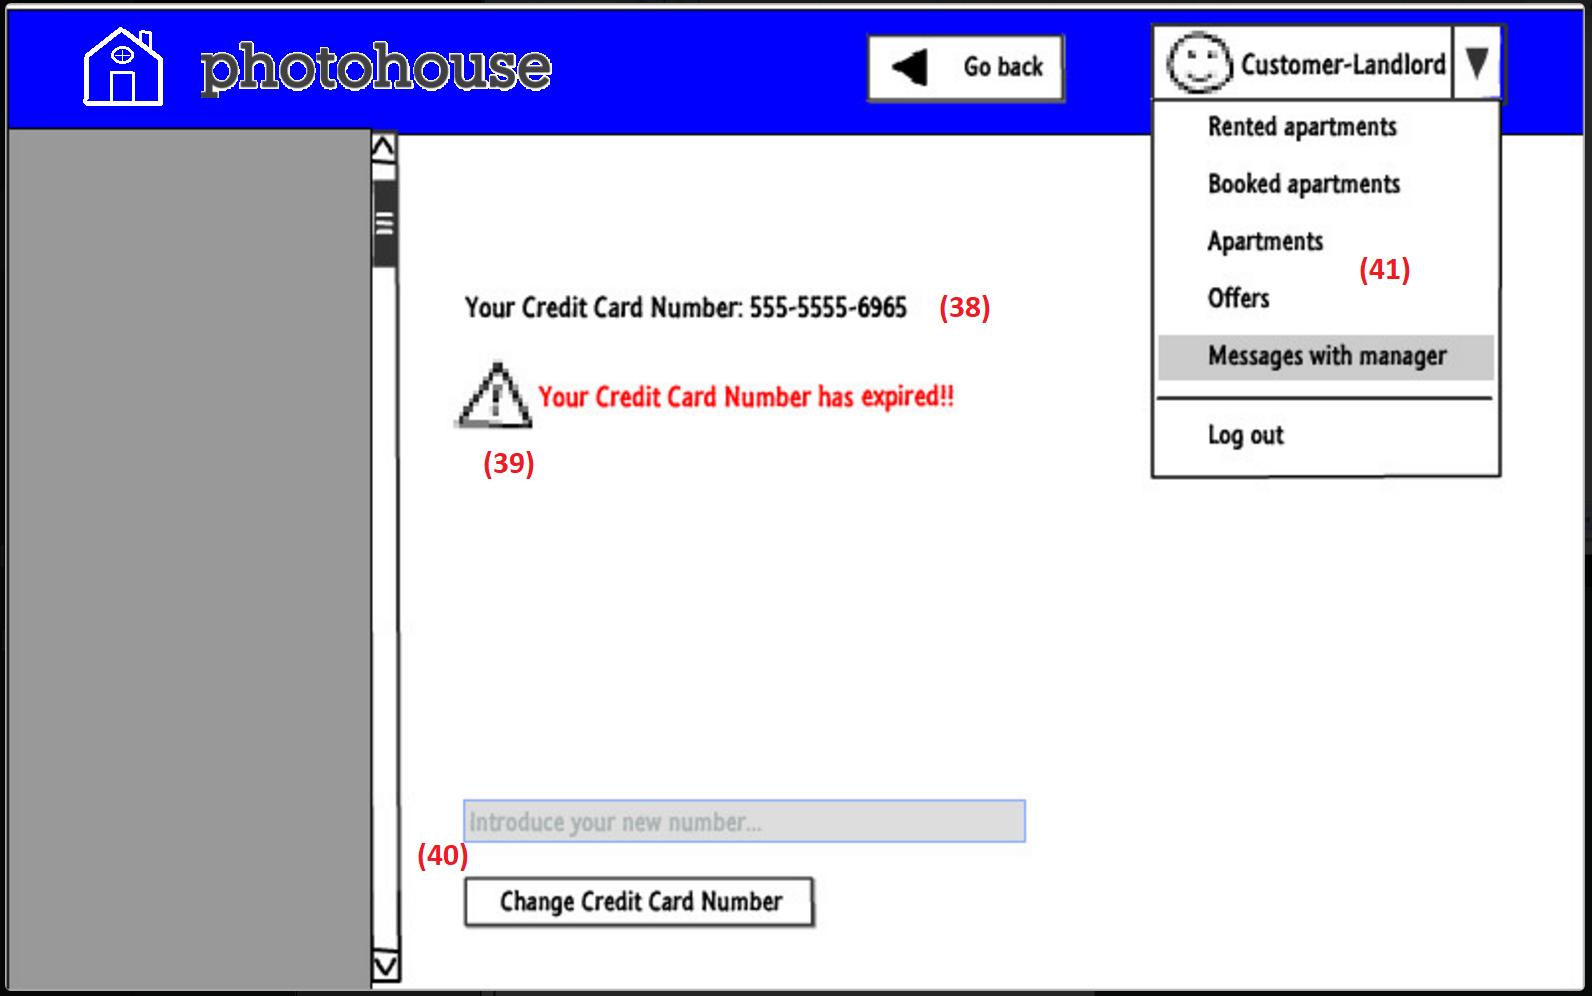
\includegraphics[scale=.7]{changing_ccn.PNG}
\end{center}


· \underline{18.-Banned as a Customer:} If you are only a Customer and your credit card is expired, you get banned from the system until you change the number. Check that you cannot do anything if you are blocked, you can't even go back \textcolor{red}{(*)}.
\begin{center}
	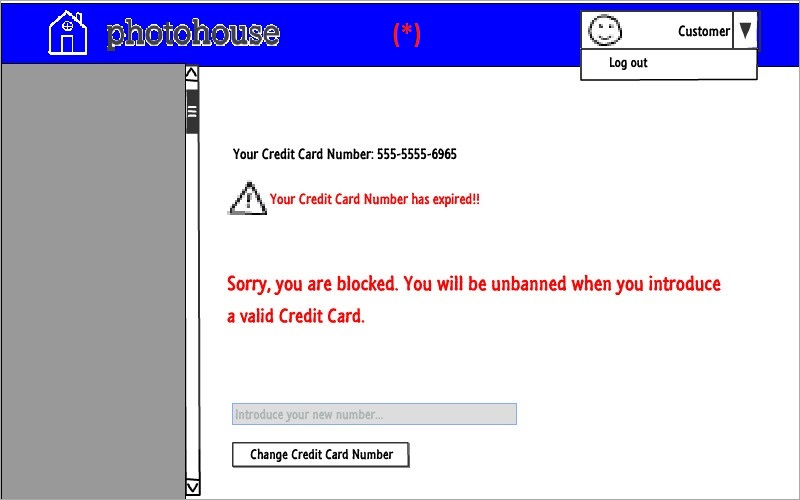
\includegraphics[scale=1.392]{customer_blocked.jpg}
\end{center}

\newpage
· \underline{19.-Login as a manager:} The manager work is to approve or deny the landlords offers \textcolor{red}{(42)} (mockup number 20), and change the credit card numbers that are requested \textcolor{red}{(43)} (mockup number 21).
\begin{center}
	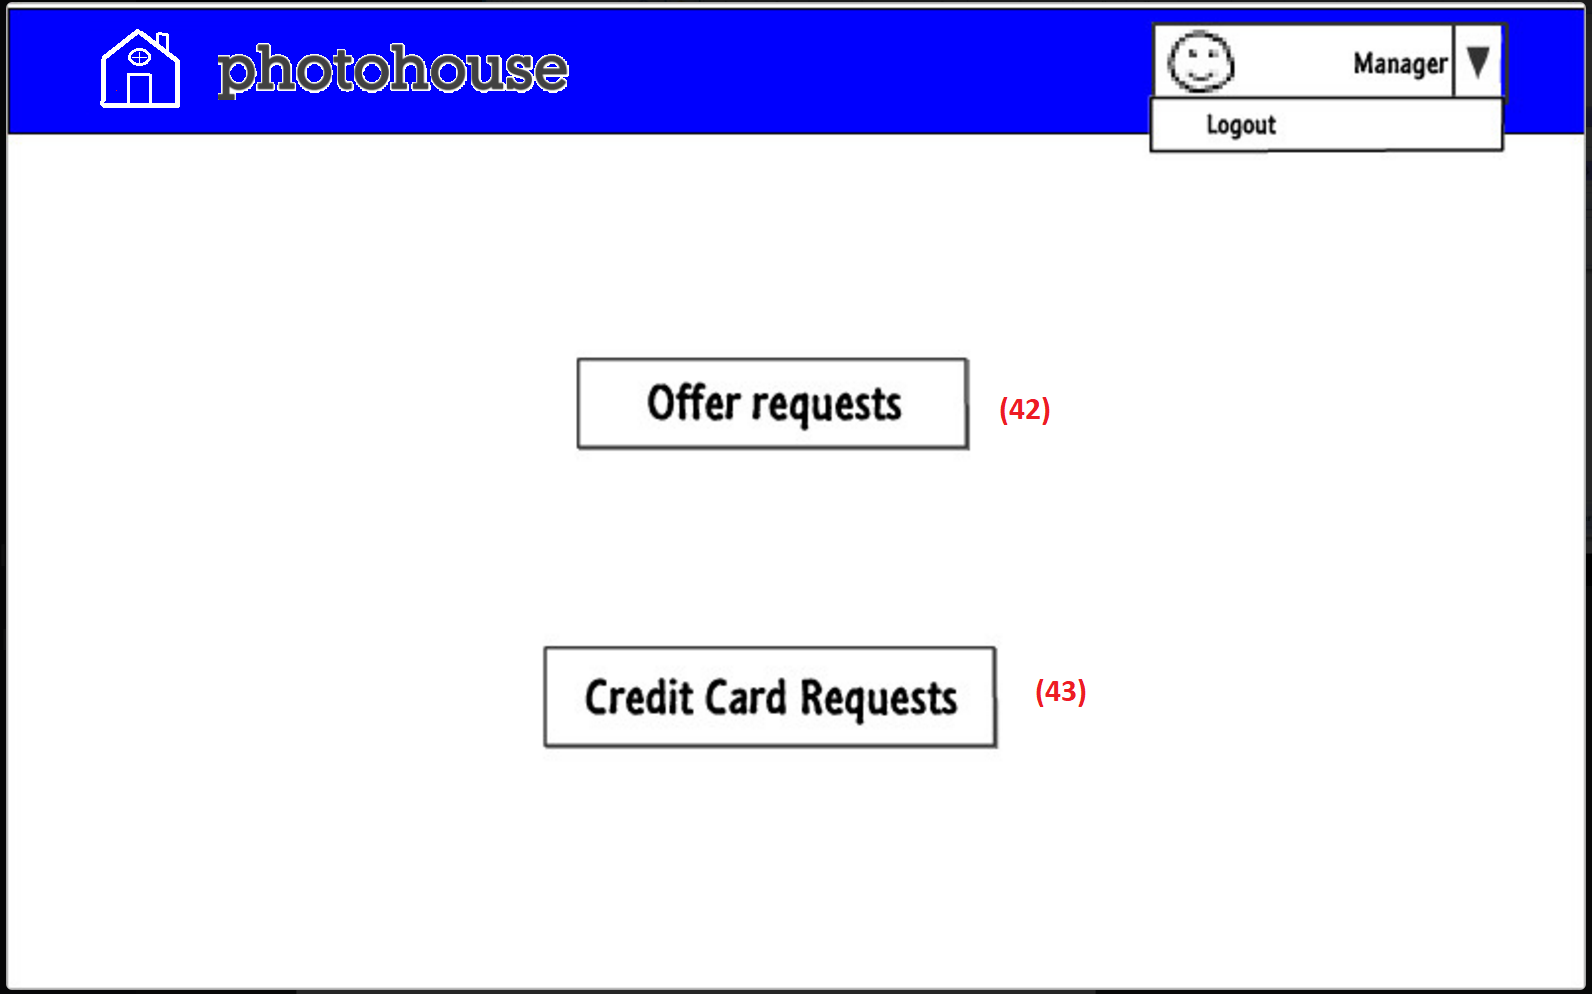
\includegraphics[scale=.7]{manager.PNG}
\end{center}


· \underline{20.-Approving or denying offers:} The manager here has to approve or deny all the offers that are requested \textcolor{red}{(44)}. In this example there is only one request, but it's supossed to apear hundreds of them.
\begin{center}
	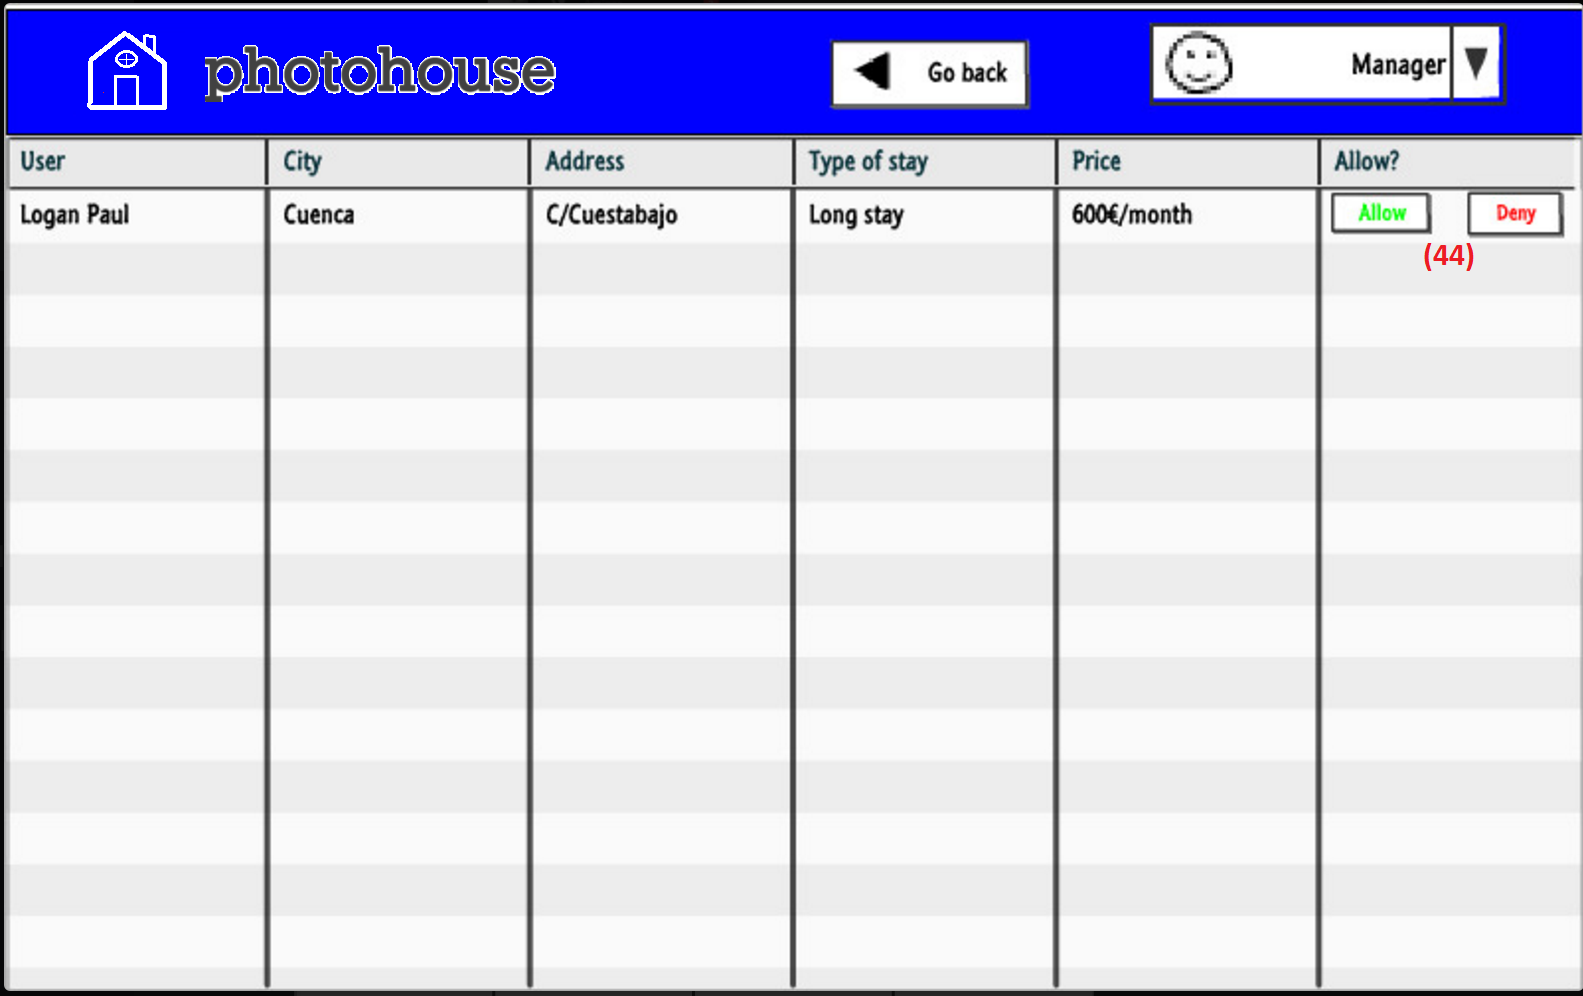
\includegraphics[scale=.7]{manager_requests.PNG}
\end{center}

\newpage
· \underline{21.-Changing credit card numbers:} The manager here has to change or to deny all the credit card numbers that are requested \textcolor{red}{(45)}. In this example there is only one request, but it's supossed to apear quite more.
\begin{center}
	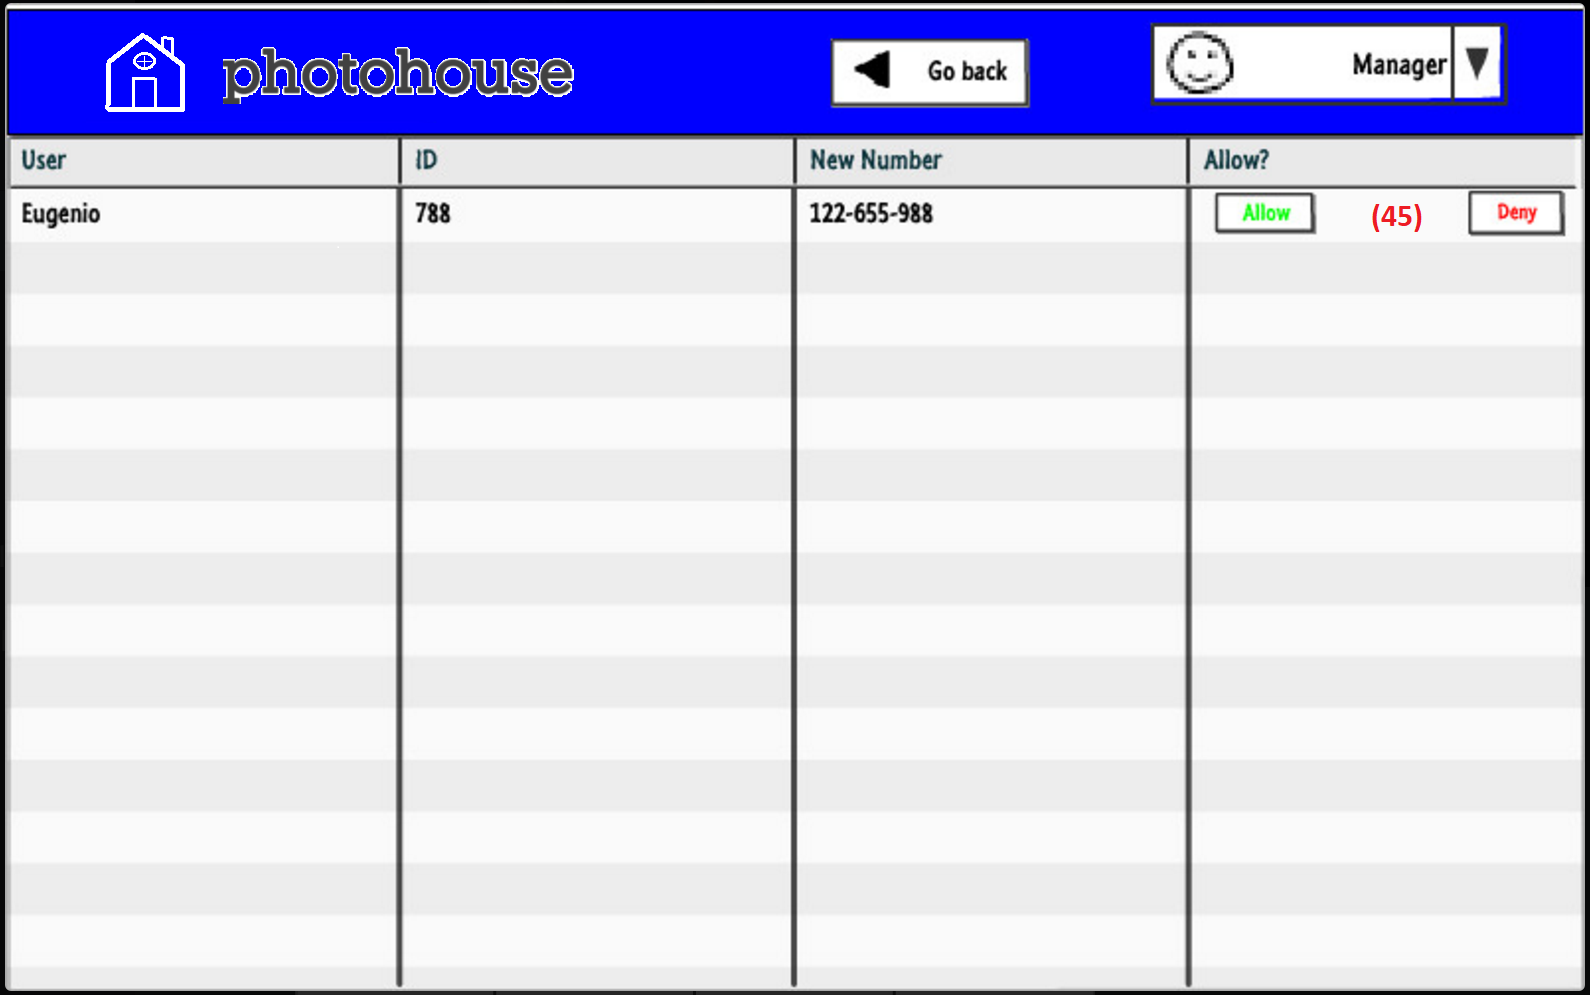
\includegraphics[scale=.7]{manager_ccn.PNG}
\end{center}

\end{document}